%%%%%%%%%%%%%%%%%%%%%%%%%%%%%%%%%%%%%%%%%%%%%%%%%%%%%%%%%%%%%%%%%%%%%%%%%
%  Zawartość: Główny plik szablonu pracy dyplomowej (magisterskiej/inżynierskiej).
%  Opracował: Tomasz Kubik <tomasz.kubik@pwr.edu.pl>
%  Data: kwiecień 2016
%  Wersja: 0.2
%%%%%%%%%%%%%%%%%%%%%%%%%%%%%%%%%%%%%%%%%%%%%%%%%%%%%%%%%%%%%%%%%%%%%%%%%



\documentclass[a4paper,onecolumn,oneside,12pt,extrafontsizes]{memoir}
% W celu przygotowania wydruku do archiwum należy przesłonić komendę powyższą
% dwoma poniższymi komendami:
%\documentclass[a4paper,onecolumn,twoside,10pt]{memoir} 
%\renewcommand{\normalsize}{\fontsize{8pt}{10pt}\selectfont}



%todonotes
\usepackage[colorinlistoftodos,prependcaption,textsize=tiny]{todonotes}
\usepackage{blindtext}


%\usepackage[cp1250]{inputenc} % jeśli kodowanie edytowanych plików to cp1250 
\usepackage[utf8]{inputenc} % jeśli kodowanie edytowanych plików to UTF8
\usepackage[T1]{fontenc}
\usepackage[polish]{babel}
%\DisemulatePackage{setspace}
\usepackage{setspace}
\usepackage{tabularx}
\usepackage{float}
\usepackage{color,calc}
%\usepackage{soul} % pakiet z komendami do podkreślania tekstu

\usepackage{ebgaramond} % pakiet z czcionkami garamond, potrzebny tylko do strony tytułowej, musi wystąpić przed pakietem tgtermes

%% Aby uzyskać polskie literki w pdfie (a nie zlepki) korzystamy z pakietu czcionek tgterms. 
%% W pakiecie tym są zdefiniowane klony czcionek Times o kształtach: normalny, pogrubiony, italic, italic pogrubiony.
%% W pakiecie tym brakuje czcionki o kształcie: slanted (podobny do italic). 
%% Jeśli w dokumencie gdzieś zostanie zastosowana czcionka slanted (np. po użyciu komendy \textsl{}), to
%% latex dokona podstawienia na czcionkę standardową i zgłosi to w ostrzeżeniu (warningu).
%% Ponadto tgtermes to czcionka do tekstu. Wszelkie matematyczne wzory będą sformatowane domyślną czcionką do wzorów.
%% Jeśli wzory mają być sformatowane z wykorzystaniem innych czcionek, trzeba to jawnie zadeklarować.

%% Po zainstalowaniu pakietu tgtermes może będzie trzeba zauktualizować informacje 
%% o dostępnych fontach oraz mapy. Można to zrobić z konsoli (jako administrator)
%% initexmf --admin --update-fndb
%% initexmf --admin --mkmaps

\usepackage{tgtermes}   
\renewcommand*\ttdefault{txtt}

% We wcześniejszej wersji szablonu korzystano z innych czcionek. Dla celów historycznych pozostawiono je w komentarzu
%\usepackage{mathptmx} % pakiet będący następcą pakietów times and mathptm, niestety polskie literki są zlepkami
%\usepackage{newtxtext,newtxmath} % pakiety dostarczające Times dla tekstów i wzorów matematycznych,  
%                                  rozwiązuje problemy występujące w mathptmx, ale wymaga zainstalowania
%                                  dodatkowych pakietów oraz uruchomienia updmap (konsola administratora)
%                                  niestety polskie literki są zlepkami
%\usepackage{newtxmath,tgtermes} % można też połączyć czcionki do tekstu i czcionki do wzorów

\usepackage{listings} % pakiet do prezentacji kodu. 
%Wcześniej był problem z polskimi znakami w otoczeniu lstlisting, stąd pozostawiono w komentarzu zastosowane wtedy rozwiązanie: 
\lstset{literate=%-
{ą}{{\k{a}}}1 {ć}{{\'c}}1 {ę}{{\k{e}}}1 {ł}{{\l{}}}1 {ń}{{\'n}}1 {ó}{{\'o}}1 {ś}{{\'s}}1 {ż}{{\.z}}1 {ź}{{\'z}}1 {Ą}{{\k{A}}}1 {Ć}{{\'C}}1 {Ę}{{\k{E}}}1 {Ł}{{\L{}}}1 {Ń}{{\'N}}1 {Ó}{{\'O}}1 {Ś}{{\'S}}1 {Ż}{{\.Z}}1 {Ź}{{\'Z}}1 }%{\ \ }{{\ }}1}

% Choć możliwe jest zastosowanie różnych pakietów formatujących tabele, zaleca się tego nie robić.
%\usepackage{longtable}
%\usepackage{ltxtable}
%\usepackage{tabulary}

%%%%%%%%%%%%%%%%%%%%%%%%%%%%%%%%%%%%%%%%%%%%%%%%%%%
%% Ustawienia odpowiedzialne za sposób łamania dokumentu
%% i ułożenie elementów pływających
%%%%%%%%%%%%%%%%%%%%%%%%%%%%%%%%%%%%%%%%%%%%%%%%%%%
%\hyphenpenalty=10000		% nie dziel wyrazów zbyt często
\clubpenalty=10000      %kara za sierotki
\widowpenalty=10000  % nie pozostawiaj wdów
\brokenpenalty=10000		% nie dziel wyrazów między stronami
\exhyphenpenalty=999999		% nie dziel słów z myślnikiem
\righthyphenmin=3			% dziel minimum 3 litery

%\tolerance=4500
%\pretolerance=250
%\hfuzz=1.5pt
%\hbadness=1450

\renewcommand{\topfraction}{0.95}
\renewcommand{\bottomfraction}{0.95}
\renewcommand{\textfraction}{0.05}
\renewcommand{\floatpagefraction}{0.35}

%%%%%%%%%%%%%%%%%%%%%%%%%%%%%%%%%%%%%%%%%%%%%%%%%%%
%%  Ustawienia rozmiarów: tekstu, nagłówka i stopki, marginesów
%%  dla dokumentów klasy memoir 
%%%%%%%%%%%%%%%%%%%%%%%%%%%%%%%%%%%%%%%%%%%%%%%%%%%
\setlength{\headsep}{10pt} 
\setlength{\headheight}{13.6pt} % wartość baselineskip dla czcionki 11pt tj. \small wynosi 13.6pt
\setlength{\footskip}{\headsep+\headheight}
\setlength{\uppermargin}{\headheight+\headsep+1cm}
\setlength{\textheight}{\paperheight-\uppermargin-\footskip-1.5cm}
\setlength{\textwidth}{\paperwidth-5cm}
\setlength{\spinemargin}{2.5cm}
\setlength{\foremargin}{2.5cm}
\setlength{\marginparsep}{2mm}
\setlength{\marginparwidth}{2.3mm}
%\settrimmedsize{297mm}{210mm}{*}
%\settrims{0mm}{0mm}	
\checkandfixthelayout[fixed] % konieczne, aby się dobrze wszystko poustawiało
%%%%%%%%%%%%%%%%%%%%%%%%%%%%%%%%%%%%%%%%%%%%%%%%
%%  Ustawienia odległości linii, wcięć, odstępów
%%%%%%%%%%%%%%%%%%%%%%%%%%%%%%%%%%%%%%%%%%%%%%%%
\linespread{1}
%\linespread{1.241}
\setlength{\parindent}{14.5pt}
%\setbeforesecskip{10pt plus 0.5ex}%{-3.5ex \@plus -1ex \@minus -.2ex}
%\setaftersecskip{10pt plus 0.5ex}%\onelineskip}
%\setbeforesubsecskip{8pt plus 0.5ex}%{-3.5ex \@plus -1ex \@minus -.2ex}
%\setaftersubsecskip{8pt plus 0.5ex}%\onelineskip}
%\setlength\floatsep{6pt plus 2pt minus 2pt} 
%\setlength\intextsep{12pt plus 2pt minus 2pt} 
%\setlength\textfloatsep{12pt plus 2pt minus 2pt} 

%%%%%%%%%%%%%%%%%%%%%%%%%%%%%%%%%%%%%%%%%%%%%%%%%%%
%%  Pakiety i komendy zastosowane tylko do zamieszczenia informacji o użytych komendach i fontach
%%  Normalnie nie są potrzebne, można je zamarkować podczas redakcji pracy
%%%%%%%%%%%%%%%%%%%%%%%%%%%%%%%%%%%%%%%%%%%%%%%%%%%
\usepackage{memlays}     % extra layout diagrams, zastosowane w szblonie do 'debuggowania', używa pakietu layouts
%\usepackage{layouts}
\usepackage{printlen} % pakiet do wyświetlania wartości zdefiniowanych długości, stosowany do 'debuggowania'
\uselengthunit{pt}
\makeatletter
\newcommand{\showFontSize}{\f@size pt} % makro wypisujące wielkość bieżącej czcionki
\makeatother
% do pokazania ramek można byłoby użyć:
%\usepackage{showframe} 


%%%%%%%%%%%%%%%%%%%%%%%%%%%%%%%%%%%%%%%%%%%%%%%%%%%
%%  Formatowanie list wyliczeniowych, wypunktowań i własnych otoczeń
%%%%%%%%%%%%%%%%%%%%%%%%%%%%%%%%%%%%%%%%%%%%%%%%%%%

% Domyślnie wypunktowania mają zadeklatorowane znaki, które nie występują w tgtermes
% Aby latex nie podstawiał w ich miejsca znaków z czcionki standardowej można zrobić podstawienie:
%    \DeclareTextCommandDefault{\textbullet}{\ensuremath{\bullet}}
%    \DeclareTextCommandDefault{\textasteriskcentered}{\ensuremath{\ast}}
%    \DeclareTextCommandDefault{\textperiodcentered}{\ensuremath{\cdot}}
% Jednak jeszcze lepszym pomysłem jest zdefiniowanie otoczeń z wykorzystaniem enumitem
\usepackage{enumitem} % pakiet pozwalający zarządzać formatowaniem list wyliczeniowych
\setlist{noitemsep,topsep=4pt,parsep=0pt,partopsep=4pt,leftmargin=*} % zadeklarowane parametry pozwalają uzyskać 'zwartą' postać wypunktowania bądź wyliczenia
\setenumerate{labelindent=0pt,itemindent=0pt,leftmargin=!,label=\arabic*.} % można zmienić \arabic na \alph, jeśli wyliczenia mają być z literkami
\setlistdepth{4} % definiujemy głębokość zagnieżdżenia list wyliczeniowych do 4 poziomów
\setlist[itemize,1]{label=$\bullet$}  % definiujemy, jaki symbol ma być użyty w wyliczeniu na danym poziomie
\setlist[itemize,2]{label=\normalfont\bfseries\textendash}
\setlist[itemize,3]{label=$\ast$}
\setlist[itemize,4]{label=$\cdot$}
\renewlist{itemize}{itemize}{4}

%%%http://tex.stackexchange.com/questions/29322/how-to-make-enumerate-items-align-at-left-margin
%\renewenvironment{enumerate}
%{
%\begin{list}{\arabic{enumi}.}
%{
%\usecounter{enumi}
%%\setlength{\itemindent}{0pt}
%%\setlength{\leftmargin}{1.8em}%{2zw} % 
%%\setlength{\rightmargin}{0zw} %
%%\setlength{\labelsep}{1zw} %
%%\setlength{\labelwidth}{3zw} % 
%\setlength{\topsep}{6pt}%
%\setlength{\partopsep}{0pt}%
%\setlength{\parskip}{0pt}%
%\setlength{\parsep}{0em} % 
%\setlength{\itemsep}{0em} % 
%%\setlength{\listparindent}{1zw} % 
%}
%}{
%\end{list}
%}

\makeatletter
\renewenvironment{quote}{
	\begin{list}{}
	{
	\setlength{\leftmargin}{1em}
	\setlength{\topsep}{0pt}%
	\setlength{\partopsep}{0pt}%
	\setlength{\parskip}{0pt}%
	\setlength{\parsep}{0pt}%
	\setlength{\itemsep}{0pt}
	}
	}{
	\end{list}}
\makeatother

%%%%%%%%%%%%%%%%%%%%%%%%%%%%%%%%%%%%%%%%%
%%  Pakiet do generowania indeksu (ważne, aby wstawić przed hyperref)
%%%%%%%%%%%%%%%%%%%%%%%%%%%%%%%%%%%%%%%%%
\DisemulatePackage{imakeidx}
\usepackage[makeindex,noautomatic]{imakeidx} % tutaj mówimy, żeby indeks nie generował się automatycznie, 

%\usepackage[noautomatic]{imakeidx} 
\makeindex

\makeatletter
%%%\renewenvironment{theindex}
							 %%%{\vskip 10pt\@makeschapterhead{\indexname}\vskip -3pt%
								%%%\@mkboth{\MakeUppercase\indexname}%
												%%%{\MakeUppercase\indexname}%
								%%%\vspace{-3.2mm}\parindent\z@%
								%%%\renewcommand\subitem{\par\hangindent 16\p@ \hspace*{0\p@}}%%
								%%%\phantomsection%
								%%%\begin{multicols}{2}
								%%%%\thispagestyle{plain}
								%%%\parindent\z@                
								%%%%\parskip\z@ \@plus .3\p@\relax
								%%%\let\item\@idxitem}
							 %%%{\end{multicols}\clearpage}
%%%
\makeatother


\usepackage{ifpdf}
%\newif\ifpdf \ifx\pdfoutput\undefined
%\pdffalse % we are not running PDFLaTeX
%\else
%\pdfoutput=1 % we are running PDFLaTeX
%\pdftrue \fi
\ifpdf
 \usepackage[pdftex,bookmarks,breaklinks,unicode]{hyperref}
 \usepackage[pdftex]{graphicx}
 \DeclareGraphicsExtensions{.pdf,.jpg,.mps,.png}
\pdfcompresslevel=9
\pdfoutput=1
\makeatletter
\AtBeginDocument{
  \hypersetup{
	pdfinfo={
    Title = {\@title},
    Author = {\@author},
    Subject={},
    Keywords={słowa kluczowe},
  }}
}
\makeatother
\else
\usepackage{graphicx}
\DeclareGraphicsExtensions{.eps,.ps,.jpg,.mps,.png}
\fi
\sloppy


%\graphicspath{{rys01/}{rys02/}}


%%%%%%%%%%%%%%%%%%%%%%%%%%%%%%%%%%%%%%%%%
% Metadane dla pdfa


%\ifpdf
%\pdfinfo{
   %/Author (Nicola Talbot)
   %/Title  (Creating a PDF document using PDFLaTeX)
   %/CreationDate (D:20040502195600)
   %/ModDate (D:\pdfdate)
   %/Subject (PDFLaTeX)
   %/Keywords (PDF;LaTeX)
%}
%\fi

% Deklaracja głębokościu numeracji
\setcounter{secnumdepth}{2}
\setcounter{tocdepth}{2}
\setsecnumdepth{subsection} % activating subsubsec numbering in doc


% Kropki po numerach sekcji
\makeatletter
\def\@seccntformat#1{\csname the#1\endcsname.\quad}
\def\numberline#1{\hb@xt@\@tempdima{#1\if&#1&\else.\fi\hfil}}
\makeatother

\renewcommand{\chapternumberline}[1]{#1.\quad}
\renewcommand{\cftchapterdotsep}{\cftdotsep}

%\definecolor{niceblue}{rgb}{.168,.234,.671}

% Czcionka do podpisów tabel i rysunków
\captionnamefont{\small}
\captiontitlefont{\small}
% makro pozwalające zmienić sposób wypisywania rozdziału
%\def\printchaptertitle##1{\fonttitle \space \thechapter.\space ##1} 

%\usepackage{ltcaption}
% The ltcaption package supports \CaptionLabelFont & \CaptionTextFont introduced by the NTG document classes
%\renewcommand\CaptionLabelFont{\small}
%\renewcommand\CaptionTextFont{\small}

% Przedefiniowanie etykiet w podpisach tabel i rysunków
%\AtBeginDocument{% 
        \addto\captionspolish{% 
        \renewcommand{\tablename}{Tab.}% 
}%} 

%\AtBeginDocument{% 
%        \addto\captionspolish{% 
%        \renewcommand{\chaptername}{Rozdział}% 
%}} 

%\AtBeginDocument{% 
        \addto\captionspolish{% 
        \renewcommand{\figurename}{Rys.}% 
}%}


%\AtBeginDocument{% 
        \addto\captionspolish{% 
        \renewcommand{\bibname}{Literatura}% 
}%}

%\AtBeginDocument{% 
        \addto\captionspolish{% 
        \renewcommand{\listfigurename}{Spis rysunków}% 
}%}

%\AtBeginDocument{% 
        \addto\captionspolish{% 
        \renewcommand{\listtablename}{Spis tabel}% 
}%}

%\AtBeginDocument{% 
        \addto\captionspolish

%%%%%%%%%%%%%%%%%%%%%%%%%%%%%%%%%%%%%%%%%%%%%%%%%%%%%%%%%%%%%%%%%%                  
%% Definicje stopek i nagłówków
%%%%%%%%%%%%%%%%%%%%%%%%%%%%%%%%%%%%%%%%%%%%%%%%%%%%%%%%%%%%%%%%%%                  
\addtopsmarks{headings}{%
\nouppercaseheads % added at the beginning
}{%
\createmark{chapter}{both}{shownumber}{}{. \space}
%\createmark{chapter}{left}{shownumber}{}{. \space}
\createmark{section}{right}{shownumber}{}{. \space}
}%use the new settings

\makeatletter
\copypagestyle{outer}{headings}
\makeoddhead{outer}{}{}{\small\itshape\rightmark}
\makeevenhead{outer}{\small\itshape\leftmark}{}{}
\makeoddfoot{outer}{\small\@author:~\@titleShort}{}{\small\thepage}
\makeevenfoot{outer}{\small\thepage}{}{\small\@author:~\@title}
\makeheadrule{outer}{\linewidth}{\normalrulethickness}
\makefootrule{outer}{\linewidth}{\normalrulethickness}{2pt}
\makeatother

% fix plain
\copypagestyle{plain}{headings} % overwrite plain with outer
\makeoddhead{plain}{}{}{} % remove right header
\makeevenhead{plain}{}{}{} % remove left header
\makeevenfoot{plain}{}{}{}
\makeoddfoot{plain}{}{}{}

\copypagestyle{empty}{headings} % overwrite plain with outer
\makeoddhead{empty}{}{}{} % remove right header
\makeevenhead{empty}{}{}{} % remove left header
\makeevenfoot{empty}{}{}{}
\makeoddfoot{empty}{}{}{}


%%%%%%%%%%%%%%%%%%%%%%%%%%%%%%%%%%%%%%%
%% Definicja strony tytułowej 
%%%%%%%%%%%%%%%%%%%%%%%%%%%%%%%%%%%%%%%
\makeatletter
%Uczelnia
\newcommand\uczelnia[1]{\renewcommand\@uczelnia{#1}}
\newcommand\@uczelnia{}
%Wydział
\newcommand\wydzial[1]{\renewcommand\@wydzial{#1}}
\newcommand\@wydzial{}
%Kierunek
\newcommand\kierunek[1]{\renewcommand\@kierunek{#1}}
\newcommand\@kierunek{}
%Specjalność
\newcommand\specjalnosc[1]{\renewcommand\@specjalnosc{#1}}
\newcommand\@specjalnosc{}
%Tytuł po angielsku
\newcommand\titleEN[1]{\renewcommand\@titleEN{#1}}
\newcommand\@titleEN{}
%Tytuł krótki
\newcommand\titleShort[1]{\renewcommand\@titleShort{#1}}
\newcommand\@titleShort{}
%Promotor
\newcommand\promotor[1]{\renewcommand\@promotor{#1}}
\newcommand\@promotor{}

%\usepackage[absolute]{textpos} % zamarkowano, bo ostatecznie wykorzystano otoczenie picture

\def\maketitle{%
  \pagestyle{empty}%
%%\garamond 
	\fontfamily{\ebgaramond@family}\selectfont % na stronie tytułowej czcionka garamond
%%%%%%%%%%%%%%%%%%%%%%%%%%%%%%%%%%%%%	
%% Poniżej, w otoczniu picture, wstawiono tytuł i autora. 
%% Tytuł (z autorem) musi znaleźć się w obszarze 
%% odpowiadającym okienku 110mmx75mm, którego lewy górny róg 
%% jest w położeniu 77mm od lewej i 111mm od górnej  krawędzi strony 
%% (tak wynika z wycięcia na okładce). 
%% Poniższy kod musi być użyty dokładnie w miejscu gdzie jest.
%% Jeśli tytuł nie mieści się w okienku, to należy tak pozmieniać 
%% parametry użytych komend, aby ten przydługi tytuł jednak 
%% upakować go do okienka.
%%
%% Sama okładka (kolorowa strona z wycięciem, do pobrania z dydaktyki) 
%% powinna być przycięta o 3mm od każdej z krawędzi.
%% Te 3mm pewnie zostawiono na ewentualne spady czy też specjalną oprawę.
%%%%%%%%%%%%%%%%%%%%%%%%%%%%%%%%%%%%%	
\newlength{\tmpfboxrule}
\setlength{\tmpfboxrule}{\fboxrule}
\setlength{\fboxsep}{2mm}
\setlength{\fboxrule}{0mm} 
%\setlength{\fboxrule}{0.1mm} %% jeśli chcemy zobaczyć ramkę
\setlength{\unitlength}{1mm}
\begin{picture}(0,0)
\put(26,-124){\fbox{
\parbox[c][71mm][c]{104mm}{\centering%\lineskip=34pt 
\fontsize{16pt}{18pt}\selectfont \@title\\[5mm]
\fontsize{16pt}{18pt}\selectfont \@titleEN\\[20mm]
\fontsize{16pt}{18pt}\selectfont AUTOR:\\[2mm]
\fontsize{14pt}{16pt}\selectfont \@author}
}
}
\end{picture}
\setlength{\fboxrule}{\tmpfboxrule} 
%%%%%%%%%%%%%%%%%%%%%%%%%%%%%%%%%%%%%
%% Reszta strony z nazwą uczelni, wydziału, kierunkiem, specjalnością
%% promotorem, oceną pracy, miastem i rokiem
	{\centering%\vspace{-1cm}
		{\fontsize{22pt}{24pt}\selectfont \@uczelnia}\\[0.4cm]
		{\fontsize{22pt}{24pt}\selectfont \@wydzial}\\[0.5cm]
		  \hrule %\vspace*{0.7cm}
	}
{\flushleft\fontsize{14pt}{16pt}\selectfont%
\begin{tabular}{ll}
KIERUNEK: & \@kierunek\\
SPECJALNOŚĆ: & \@specjalnosc\\
\end{tabular}\\[1.3cm]
}
{\centering
{\fontsize{32pt}{36pt}\selectfont PRACA DYPLOMOWA}\\[0.5cm]
{\fontsize{32pt}{36pt}\selectfont INŻYNIERSKA}\\[2.5cm]
}
\vfill
\begin{tabularx}{\linewidth}{p{6cm}l}
		&{\fontsize{16pt}{18pt}\selectfont PROWADZĄCY PRACĘ:}\\[2mm] %UWAGA: tutaj jest miejsce na nazwisko promotora pracy
		&{\fontsize{14pt}{16pt}\selectfont \@promotor}\\[10mm]
		&{\fontsize{16pt}{18pt}\selectfont OCENA PRACY:}\\[20mm]
	\end{tabularx}
\vspace{2cm}
\hrule\vspace*{0.3cm}
{\centering
{\fontsize{16pt}{18pt}\selectfont \@date}\\[0cm]
}
%\ungaramond
\normalfont
 \cleardoublepage
}
\makeatother
%%%%%%%%%%%%%%%%%%%%%%%%%%%%%%%%%%%%%%%%%

%\AtBeginDocument{\addtocontents{toc}{\protect\thispagestyle{empty}}}




%%%%%%%%%%%%%%%%%%%%%%%%%%%%%%%%%%%%%%%%%
%%  Metadane dokumentu 
%%%%%%%%%%%%%%%%%%%%%%%%%%%%%%%%%%%%%%%%%
\title{Aplikacja webowa służąca do układania diety}
\titleShort{Projekt i implementacja aplikacji webowej służącej do układania diety}
\titleEN{Design and implementation of a web application for diet planning}
\author{Janusz Długosz}
\uczelnia{POLITECHNIKA WROCŁAWSKA}
\wydzial{WYDZIAŁ ELEKTRONIKI}
\kierunek{INFORMATYKA}
\specjalnosc{SYSTEMY I SIECI KOMPUTEROWE}
\promotor{dr inż., Wojciech Kmiecik, W4K2}
\date{WROCŁAW, 2019}

% Ustawienie odstępu od góry w nienumerowanych rozdziałach oraz wykazach:
% Spis treści, Spis tabel, Spis rysunków, Indeks rzeczowy

%\newlength{\linespace}
%\setlength{\linespace}{-\beforechapskip-\topskip+\headheight+\topsep}
%\makechapterstyle{noNumbered}{%
%\renewcommand\chapterheadstart{\vspace*{\linespace}}
%}

%% powyższa komenda załatwia to, co robią komendy poniższe dla spisów
%\renewcommand*{\tocheadstart}{\vspace*{\linespace}}
%\renewcommand*{\lotheadstart}{\vspace*{\linespace}}
%\renewcommand*{\lofheadstart}{\vspace*{\linespace}}

%%%%%%%%%%%%%%%%%%%%%%%%%%%%%%%%%%%%%%%%%
%                  Początek dokumentu 
%%%%%%%%%%%%%%%%%%%%%%%%%%%%%%%%%%%%%%%%%
%\includeonly{skroty,rozdzial01} % jeśli chcemy kompilować tylko fragmenty, to można tu je wpisać

\begin{document}
% Tutaj można przełączyć odstęp między liniami
%\SingleSpacing
%\OnehalfSpacing
%\DoubleSpacing
%listningi
\lstdefinestyle{mystyle}{frame=single}    
\lstset{style=mystyle}
\lstdefinelanguage{JavaScript}{
  morekeywords={typeof, new, true, false, catch, function, return, null, catch, switch, var, if, in, while, do, else, case, break},
  morecomment=[s]{/*}{*/},
  morecomment=[l]//,
  morestring=[b]",
  morestring=[b]'
}

\lstdefinelanguage{HTML5}{
        language=html,
        sensitive=true, 
        alsoletter={<>=-},
        otherkeywords={
        % HTML tags
        <html>, <head>, <title>, </title>, <meta, />, </head>, <body>,
        <canvas, \/canvas>, <script>, </script>, </body>, </html>, <!, html>, <style>, </style>, ><
        },  
        ndkeywords={
        % General
        =,
        % HTML attributes
        charset=, id=, width=, height=,
        % CSS properties
        border:, transform:, -moz-transform:, transition-duration:, transition-property:, transition-timing-function:
        },  
        morecomment=[s]{<!--}{-->},
        tag=[s]
}

%\settypeoutlayoutunit{cm} % do debugowania
%\typeoutstandardlayout    % wypisuje na stdout informacje o ustawieniach
\maketitle

\newpage



\chapterstyle{noNumbered}
\pagestyle{outer}
\mbox{}\pdfbookmark[0]{Spis treści}{spisTresci.1}
\tableofcontents* 



\include{skroty} %skróty można sobie pominąć
\chapterstyle{default}
\chapter{Wstęp}
\section{Cel i zakres pracy}
Celem pracy jest zaprojektowanie i zaimplementowanie aplikacji internetowej służącej do pomagania w układaniu diety na podstawie dziennego zapotrzebowania kalorycznego użytkownika. Powodem powstania tej pracy jest niska wiedza i świadomość ludzi w dziedzinie zdrowego oraz zbilansowanego żywienia.\cite{zywienie} Poza tym wpływ na wybór technologii miały zainteresowania autora, chęć podniesienia własnych umiejętności oraz obecne trendy.\cite{stack} Aplikacja ma działać na każdej współczesnej przeglądarce internetowej. Backend został wykonany na platformie ASP.NET Core 3.0, frontend w Angular 8.0, natomiast jako baza danych wykorzystywało  PostgreSQL 11.4. API oparte zostało na otwartym standardzie GraphQL. W zakres pracy wchodzi:
\begin{itemize}
    \item zapoznanie się z potrzebnymi bibliotekami i platformami programistycznymi,
    \item analiza potrzeb funkcjonalnych i niefunkcjonalnych użytkowników,
    \item projekt i konfiguracja bazy danych,
    \item projekt aplikacji,
    \item instrukcja użytkowania,
    \item krótka analiza wydajności aplikacji,
    \item testowanie aplikacji.
\end{itemize}
\section{Układ pracy}
\todo{Na końcu zrobić}



\chapter{Przegląd i analiza istniejących rozwiązań}
\label{chap:technologies}
W poniższym rozdziale zostały przedstawione wykorzystane technologie. Zostały one dobrane w taki sposób, aby ułatwić stworzenie funkcjonalnej i łatwo rozszerzalnej aplikacji przeglądarkowej.
\section{GraphQL}

GraphQL jest otwartym standardem języka kwerendowego przeznaczonym do budowania API dla różnorakich aplikacji. Obecnie został zaimplementowany w wielu językach\cite{gqlcode}, również w C\# oraz JavaScripcie, które będę wykorzystywane w budowaniu programu. GraphQL nie jest związany z żadną konkretną bazą danych czy rozwiązaniem do przechowywania informacji. Serwisy są tworzone poprzez definiowanie typów oraz ich pól, a następnie funkcji dla każdego pola. Jako całość tworzą schemat GraphQL. Bardzo ważne jest, aby stworzyć ją na samym początku i nie edytować jej nadto, ponieważ stanowi ona ,,kontrakt'' między frontendem, a backendem, definiując w jaki sposób klient ma dostęp do danych. Ma to duże znaczenie w większych projektach, ponieważ zespoły mogą pracować od siebie niezależnie znając strukturę danych. Przykładem typu i funkcji zwracającej przykładowy typ:
\begin{lstlisting}[language=sh]
type Query {
  getUser: User
}

type User {
  id: ID
  name: String
}
\end{lstlisting}
Kiedy serwis GraphQL jest już uruchomiony, można wysyłać do niego kwerendy do walidacji, a następnie wykonania. Komunikacja przebiega w oparciu o standard JSON. Przykładowa kwerenda może wyglądać w następujący sposób:
\begin{lstlisting}[language=sh]
{
  getUser {
    name
  }
}
\end{lstlisting}
Wywołanie jej da następujący rezultat:
\begin{lstlisting}[language=sh]
{
  "getName": {
    "name": "Johhny"
  }
}
\end{lstlisting}
W odróżnienia od szeroko stosowanej technologii REST w GraphQL wystawiany jest tylko jeden endpoint, który odbiera wszystkie kwerendy i mutacje. Dzięki temu można definiować w bardzo elastyczny sposób dane, które chcemy pobrać i nie ma problemu sztywno określonych typów zwracanych, co może prowadzić to dostawania niewystarczającej lub za dużej ilości danych, co występuje w konkurencyjnym rozwiązaniu.

\section{PostgreSQL}
PostgreSQL jest darmową i otwarto-źródłową relacyjną bazą danych. Została stworzona do obsługiwania małego obciążenia jak i dużego oraz wielu użytkowników używającej jej współbieżnie. Jest dostępna na praktycznie większość obecnie używanych systemów (w tym np. Linux, Windows, macOS). Charakteryzuje się ona wysoką stabilnością i stosunkowo niskim wykorzystaniem zasobów. PostgreSQL oferuje wiele zaawansowanych funkcjonalności takich jak: 
\begin{itemize}
    \item możliwość zdefiniowania przez użytkownika typów,
    \item dziedziczenie tabel,
    \item bardzo dobry mechanizm blokowania danych,
    \item integralność referencyjna kluczy obcych,
    \item widoki,
    \item indeksy,
    \item funkcje,
    \item zasady,
    \item podkwerendy,
    \item mechanizm kontroli współbieżności (ang. Multiversion Concurrency Control), pozwalający na jednoczesny dostęp oraz wykonywanie operacji różnym użytkownikom,
    \item zagnieżdżone transakcje,
    \item mechanizm asynchronicznej replikacji,
    \item dowolna rozszerzalność, dzięki możliwości pisania wtyczek.
\end{itemize}
Zwłaszcza mechanizm kontroli współbieżności okazuje się bardzo przydatny w budowie aplikacji, z której będzie możliwość korzystania przez wielu użytkowników naraz, czyli np. aplikacji, którą omawia niniejsza praca. Oszczędza to wiele czasu, ponieważ nie trzeba ręcznie budować skomplikowanego systemu, który by to obsłużył albo zostawić aplikację niedopracowaną. PostgreSQL posiada również dobrą integrację z Entity Framework Core, który używany jest do zarządzania bazą danych w projekcie.

\section{ASP .NET Core}
ASP .NET Core jest międzyplatformową, wydajną, otwarto-źródłową platformą programistyczną wykorzystywaną do budowania nowoczesnych aplikacji internetowych oraz API. Wykorzystuje on wzorzec projektowy MVC (ang. Model-View-Controller), który pozwala na usystematyzowanie i oddzielenie części składowych aplikacji, co oprócz zwiększania czytelności kodu oraz modularności programu, pozwala na uporządkowane testowanie. Framework wykorzystuje również Razor Pages, które pozwalają na tworzenie interfejsu użytkownika, ale z powodzeniem można to zastąpić innymi technologiami frontendowymi takimi jak:
\begin{itemize}
    \item Angular,
    \item React,
    \item Bootstrap.
\end{itemize}
ASP .NET Core posiada wiele cech, które wyróżniają go na tle innych rozwiązań, a są nimi:
\begin{itemize}
    \item ciągła kompilacja, czyli brak konieczności rekompilowania całego projektu po dokonaniu jakiejkolwiek zmiany,
    \item modularna budowa, dzięki bibliotekom, których instalacja jest prosta dzięki menadżerowi pakietów NuGet,
    \item cykl działania programu zoptymalizowany pod użycie w chmurze,
    \item łatwa konfiguracja uruchomieniowa w chmurze,
    \item lekki i modularny potok żądań HTTP,
    \item możliwość działania na systemach Windows, Linux oraz Mac,
    \item otwarto-źródłowa,
    \item skupiony na społeczności,
    \item wbudowany mechanizm wstrzykiwania zależności,
    \item mechanizmy automatycznej walidacji po stronie klienta oraz serwera.
\end{itemize}
W projekcie inżynierskim został on wykorzystany w formie backendu. Dzięki gotowym bibliotekom implementującym standard GraphQL, Identity Core oraz biblioteką Entity Framework Core wraz z dodatkiem do obsługi bazy danych PostgreSQL pełni kilka kluczowych funkcji:
\begin{itemize}
    \item wystawienie endpointu dla frontendu,
    \item operacje związane z komunikacją z bazą danych (pobieranie, dodawanie, edycja, usuwanie),
    \item definicja struktury bazy danych (podejście Code First, czyli generowanie tabel i relacji bazy danych na podstawie kodu),
    \item definicja schematu (typy, kwerendy, mutacje) GraphQL,
    \item obliczenia,
    \item walidacje,
    \item filtrowania,
    \item zarządzanie użytkownikami (rejestracja, logowanie).
\end{itemize}

\subsection{Entity Framework Core}
Jest to biblioteka, która służy do obsługi różnych baz danych w tym PostgreSQL. Entity Framework Core służy również do mapowania obiektowo-relacyjnego, która pozwala na odwzorowanie struktury obiektowej programu na relacyjną bazę danych.\cite{efcore} Podejście takie pozwala na bezpośrednie odwoływanie się do bazy danych przez obiekty, nie ma potrzeby pisania skomplikowanych kwerend SQL-owych. Aby dokonać mapowania niezbędne jest utworzenie modelów wszystkich obiektów. Na przykład w poniższy sposób:
\begin{lstlisting}[language={[Sharp]C}]
public class Blog
    {
        public int BlogId { get; set; }
        public string Url { get; set; }
        public int Rating { get; set; }
        public List<Post> Posts { get; set; }
    }

    public class Post
    {
        public int PostId { get; set; }
        public string Title { get; set; }
        public string Content { get; set; }

        public int BlogId { get; set; }
        public Blog Blog { get; set; }
    }
\end{lstlisting}
Dzięki językowi LINQ można w łatwy i w o wiele bardziej czytelny niż standardowy język SQL, wykonywać kwerendy. Na przykład w taki sposób:
\begin{lstlisting}[language={[Sharp]C}]
   using (var db = new BloggingContext())
{
    var blogs = db.Blogs
        .Where(b => b.Rating > 3)
        .OrderBy(b => b.Url)
        .ToList();
}
\end{lstlisting}
Zapisywanie danych również jest bajecznie proste, wystarczy stworzyć nowy obiekt, dodać go do odpowiedniej tabeli i wykonać metodę \texttt{SaveChanges()}:
\begin{lstlisting}[language={[Sharp]C}]
using (var db = new BloggingContext())
{
    var blog = new Blog { Url = "http://sample.com" };
    db.Blogs.Add(blog);
    db.SaveChanges();
}
\end{lstlisting}

\subsection{Identity Core}
Jest to biblioteka obsługująca system zarządzania tożsamością. Główna funkcjonalność obejmuje:
\begin{itemize}
    \item integracja z relacyjną bazą danych lub z Azure Table Storage w celu przechowywania danych użytkownika,
    \item zarejestrowanie nowego użytkownika i dodanie go do bazy,
    \item wspieranie logowania się poprzez konta Facebook, Google, Microsoft oraz Twitter,
    \item uwierzytelnianie oraz autoryzacja,
    \item obsługa OpenID Connect oraz OAuth 2.0,
    \item gotowy interfejs graficzny użytkownika.
\end{itemize}

\section{Angular}
Jest platformą programistyczną wykorzystywaną do budowania klientów aplikacji w HTML oraz TypeScript.\cite{angulararch} Angular sam w sobie został napisany w języku TypeScript, dzięki temu zawiera wszystkie jego funkcjonalności i biblioteki. Podstawowym elementem, z którego budowana jest aplikacja w Angularze, jest \textit{NgModule}. Zawiera ona w sobie komponenty. Aplikacja musi zawierać co najmniej jeden taki moduł. Jednak lepszym rozwiązaniem jest zaprojektowanie wiele takich modułów, ponieważ ułatwiają one organizację oraz rozbudowę. Komponenty zaś definiują widoki, które są zbiorem elementów, które Angular może wybierać i modyfikować na podstawie danych oraz logiki programu. Serwisy są używane przez komponenty w przypadkach, kiedy jakaś funkcjonalność nie jest powiązana konkretnie z jednym widokiem i może być użyta równie dobrze w jakimś innym. Dostarczane one są poprzez wstrzykiwanie zależności. Zarówno komponenty jak i serwisy są zwykłymi klasami z dekoratorami, które oznaczają ich typ oraz zapewniają odpowiednie metadane dzięki którym Angular wie jak je wykorzystać. Metadane komponentu powiązane są z szablonem, który definiuje widok, w którego skład wchodzi zwykły HTML z Angularowymi dyrektywami oraz znacznikami wiążącymi, które pozwalają na edycję danych przed ich wyświetleniem. Metadane serwisu dostarczają Angularowi informacje, które pozwalają serwisowi na stanie się dostępnym dla komponentów poprzez mechanizm wstrzykiwania zależności. Komponenty powinny definiować wiele widoków w sposób hierarchiczny. Angular dostarcza serwis \textit{Router}, który pozwala na prostą nawigację między widokami poprzez URL. Dodatkowo pozwala na przekazywanie w URL-u danych, takich jak na przykład numer identyfikacyjny jakiegoś obiektu.

Aplikacja wykorzystuje klienta Apollo do integracji z GraphQL. Pozwala on na generacje wszystkich potrzebnych typów, kwerend, mutacji ze schematu. Dzięki temu można w prosty sposób korzystać z API.

\chapter{Analiza wymagań aplikacji}
Proces analizy wymagań to kluczowy moment w etapie projektowania aplikacji, który ma na celu usystematyzowanie wymagań klienta, a następnie ich analizę. Jej celem jest sformułowanie zakresu pracy, określenie czasu potrzebnego na wykonanie projektu, a także kosztów, które się z tym wiążą. 
\cite{analiza}

\section{Wymagania funkcjonalne}
Wymagania funkcjonalne definiują w jaki sposób powinna reagować aplikacja bez określania z góry konkretnej technologii, struktury czy też implementacji. Zostały one zaprojektowane w postaci historyjek użytkownika. Jest to bardzo prosta i przystępna forma definiowania wymagań.
\newline
W aplikacji, która jest przedmiotem tej pracy, został wyszczególniony tylko jeden rodzaj użytkownika. Jest to zarejestrowany użytkownik, który wcześniej podał wymagane dane. Ma on dostęp do przeglądania wszystkich przepisów oraz może wykonywać wszystkie możliwe operacje. W aplikacji nie występuje podział na zarejestrowanych i niezarejestrowanych użytkowników, gdyż baza przepisów z założenia ma być budowana przez społeczność, a danie możliwości dodawania nowych receptur byłaby bardzo nierozważna. 
\newline
Poniżej znajdują się historyjki napisane z punktu widzenia użytkownika, które ukazują funkcjonalność aplikacji.
\begin{itemize}
    \item Jako użytkownik chcę na podstawie mojego uwarunkowania fizjologicznego (wzrost, waga, płeć) oraz zadanej ilości posiłków otrzymać listę przepisów, które spełniają moje wymagania.
    \item Jako użytkownik chcę mieć możliwość dodawania nowych przepisów.
    \item Jako użytkownik chcę mieć możliwość dodawania nowych składników, z które można wykorzystać w przepisach.
    \item Jako użytkownik chcę mieć możliwość przeglądania dodanych przeze mnie i innych użytkowników przepisów oraz szczegółów konta.
    \item Jako użytkownik chcę mieć możliwość komentowania przepisów.
    \item Jako użytkownik chcę mieć możliwość oceniania przepisów oraz komentarzy.
    \item Jako użytkownik chcę mieć wyświetlane dane w czytelny i przyjazny sposób.
\end{itemize}

\section{Wymagania niefunkcjonalne}
Wymagania niefunkcjonalne są wymaganiami, które opisują wydajność, niezawodność, bezpieczeństwo oraz właściwości aplikacji.\cite{analiza}
Poniżej znajdują się owe wymagania.
\begin{enumerate}
    \item Aplikacja, będąc aplikacją webową, powinna działać i wyglądać możliwie jak najbardziej podobnie na jak największej ilości obecnie stosowanych nowoczesnych przeglądarkach, tj. Chrome, Firefox, Edge, IE, IE Mobile, Safari, iOS, Android. Powinna też w razie wyjścia nowszych przeglądarek być w łatwy sposób przenoszalna.
    \item Aplikacja powinna przechowywać dane użytkowników w sposób bezpieczny. Tak aby osoby nieupoważnione nie miały do nich dostępu.
    \item Aplikacja powinna uwierzytelniać użytkownika podczas procesu logowania.
    \item Ze względu na jeden typ użytkownika aplikacja nie potrzebuje autoryzacji poprzez role.
    \item W przypadku braku internetu aplikacja nie powinna działać.
    \item Dane niejawne użytkowników, czyli przede wszystkim hasło, powinny być przechowywane w osobnej bazie danych.
\end{enumerate}
\section{Diagram przypadków użycia użytkownika}
Rysunek \ref{fig:use_case} obrazuje diagram przypadków użycia dla użytkownika. Przedstawione przypadki użycia pokrywają główną funkcjonalność aplikacji.

\begin{figure}[h]
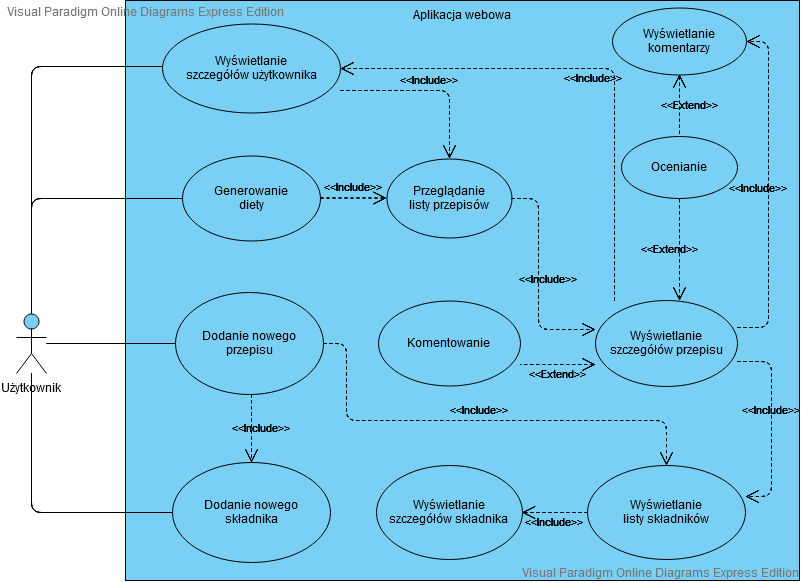
\includegraphics[width=\textwidth]{rys/use-case.png}
\caption{Diagram przypadków użycia}
\label{fig:use_case}
\end{figure}

Poniżej znajduje się krótki opis dla przypadków użycia dla przypadków przedstawionych na rysunku \ref{fig:use_case}.

\begin{enumerate}
    \item Wyświetlanie szczegółów użytkownika\newline
    Przypadek użycia dotyczący wyświetlania informacji dotyczących użytkownika takich jak:
    \begin{itemize}
        \item login,
        \item email,
        \item imię,
        \item nazwisko,
        \item płeć,
        \item data rejestracji,
        \item data ostatniej aktywności.
    \end{itemize}
    
    \item Generowanie diety\newline
    Przypadek użycia dotyczący generowania listy przepisów na podstawie:
    \begin{itemize}
        \item płci,
        \item wzrostu,
        \item wagi.
    \end{itemize}
    
    \item Dodawanie nowego przepisu\newline
    Przypadek użycia dotyczący operacji stworzenia nowego przepisu w systemie. Aby stworzyć przepis należy podać:
    \begin{itemize}
        \item nazwę,
        \item ilość kalorii,
        \item wagę,
        \item opis,
        \item listę składników,
        \item poziom trudności,
        \item szacowany czas przygotowania.
    \end{itemize}
    Utworzenie nowego przepisu w aplikacji jest równoznaczne z dodaniem go w bazie danych.
    
    \item Dodanie nowego składnika\newline
    Przypadek użycia dotyczący operacji stworzenia nowego składnika, który może być później używany w tworzeniu nowych przepisów. Aby stworzyć składnik należy podać:
    \begin{itemize}
        \item nazwę,
        \item opis,
        \item typ składnika,
        \item ilość kalorii na 100 gramów.
    \end{itemize}
    Utworzenie nowego składnika w aplikacji jest równoznaczne z dodaniem go w bazie danych.
    
    \item Przeglądanie listy przepisów\newline
    Przypadek użycia dotyczący wyświetlania listy przepisów. Lista powinna być spójna z szatą graficzną oraz zawierać możliwość paginacji, aby nie była wyświetlana zbyt duża ilość danych. Po wybraniu przepisu z listy powinny zostać wyświetlone jego szczegóły.
    
    \item Komentowanie\newline
    Przypadek użycia dotyczący dodawania komentarzy do przepisu. Wywoływany podczas wyświetlania szczegółów przepisu. Utworzenie nowego komentarza jest równoznaczne z dodaniem go w bazie danych i nie można go później usunąć.
    
    \item Wyświetlanie szczegółów składnika\newline
    Przypadek użycia dotyczący wyświetlania szczegółów składnika, który został wybrany do pokazania przez użytkownika. Powinien zawierać te same dane, które są podawane przy jego wcześniejszym dodawaniu.
    
    \item Wyświetlanie komentarzy\newline
    Przypadek użycia dotyczący wyświetlania komentarzy do przepisu. Komentarze powinny być wyświetlane w prostokątach, a liczba kolumn, w których będą pogrupowane powinna zależeć od wielkości okna przeglądarki. Komentarz powinien zawierać: 
    \begin{itemize}
        \item login użytkownika, który go dodał,
        \item treść,
        \item datę dodania,
        \item ocenę użytkowników.
    \end{itemize}
    
    \item Wyświetlanie szczegółów przepisu\newline
    Przypadek użycia dotyczący wyświetlania szczegółów przepisu, który mógł zostać wygenerowany i wybrany jako jeden z elementów składowych diety albo wybrany jako przepis dodany przez wcześniej oglądanego użytkownika. Powinien zawierać te same dane, które są podawane przy jego wcześniejszym dodawaniu oraz dodatkowo ocenę użytkowników.

    \item Ocenianie\newline
    Przypadek użycia dotyczący ocenianiu przez społeczność przepisów oraz komentarzy. Polega na oddaniu głosu pozytywnego lub negatywnego. System powinien nie zezwalać użytkownikowi na powtórne ocenienie tego samego elementu.
    
    \item Wyświetlanie listy składników\newline
    Przypadek użycia dotyczący wyświetlania listy składników. Lista powinna być spójna z szatą graficzną oraz zawierać możliwość paginacji, aby nie była wyświetlana zbyt duża ilość danych. Po wybraniu składnika z listy powinny zostać wyświetlone jego szczegóły.
\end{enumerate}
\chapter{Projektowanie aplikacji}
Proces projektowania aplikacji jest fazą, w której planowane są kwestie jak ma zostać zbudowana aplikacja, aby spełnić wszystkie wcześniej założone wymagania funkcjonalne oraz niefunkcjonalne. 

\section{Model informacyjny}
Na podstawie założeń zawartych w poprzednich rozdziałach został zaprojektowany model informacyjny zaprezentowany na Rysunku \ref{fig:db}. Będzie on niezbędny w implementacji bazy danych.

\begin{figure}[H]
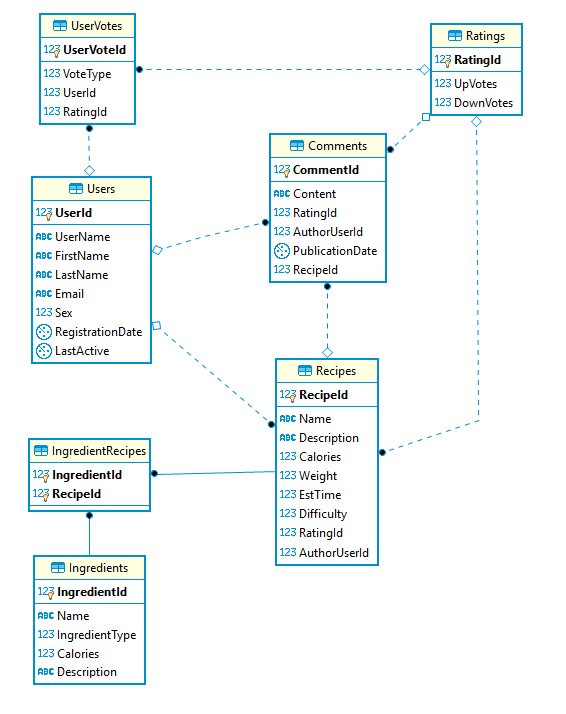
\includegraphics[width=\textwidth]{rys/db.png}
\caption{Model informacyjny aplikacji}
\label{fig:db}
\end{figure}

Najważniejszym elementem schematu jest przepis (encja \textit{Recipes}), który zawiera nazwę i opis w postaci tekstowej. Poza tym zawiera liczbę kalorii, wagę, szacowany czas w postaci liczb. Poziom trudności jest typem wyliczeniowym, więc w bazie danych będzie de facto przechowywany w postaci liczby. Kolejnym bardzo ważnym elementem są klucze obce do encji użytkownika oraz oceny.\newline
Następnym elementem jest ocena (encja \textit{Ratings}), która zawiera głosy negatywne oraz pozytywne.\newline
Kolejny jest komentarz (encja \textit{Comments}), która zawiera treść w postaci tekstu, datę publikacji, klucz obcy do autora wpisu, oceny oraz przepisu, do którego się odwołuje.\newline
Następnym elementem jest głos użytkownika (encja \textit{UserVotes}), który zawiera w sobie rodzaj głosu (negatywny lub pozytywny) i klucze obce do użytkownika, który oddał głos oraz do oceny, do której się odnosi.\newline
Dalszym w kolejności elementem jest użytkownik (encja \textit{Users}), który przechowuje szczegóły dotyczące użytkownika, takie jak nazwa użytkownika, imię, nazwisko, email, płeć, datę rejestracji oraz ostatnią aktywność. Nie przechowuje za to haseł, ponieważ powinny być przechowywane oddzielnie od danych aplikacji.\newline
Kolejnym elementem jest składnik (encja \textit{Ingredients}. Zawiera on w sobie nazwę, typ składnika, liczbę kalorii na 100 gramów oraz opis.\newline
Między przepisami, a składnikami występuje relacja wiele do wielu, aby możliwa była późniejsza implementacja tej struktury, potrzebna jest dodatkowa encja wiążąca je razem. Nazwana została \textit{IngredientRecipes} i łączy ona klucze składników z kluczami przepisów.

\section{Architektura logiczna}
\label{chap:arch_log}
Architektura logiczna aplikacji w głównej mierze wynika z technologii, która została użyta w implementacji. Na Rysunku \ref{fig:arch_log} została przedstawiony jej schemat. Warstwa logiki została wyraźnie oddzielona od warstwy klienta.\newline

\begin{figure}[H]
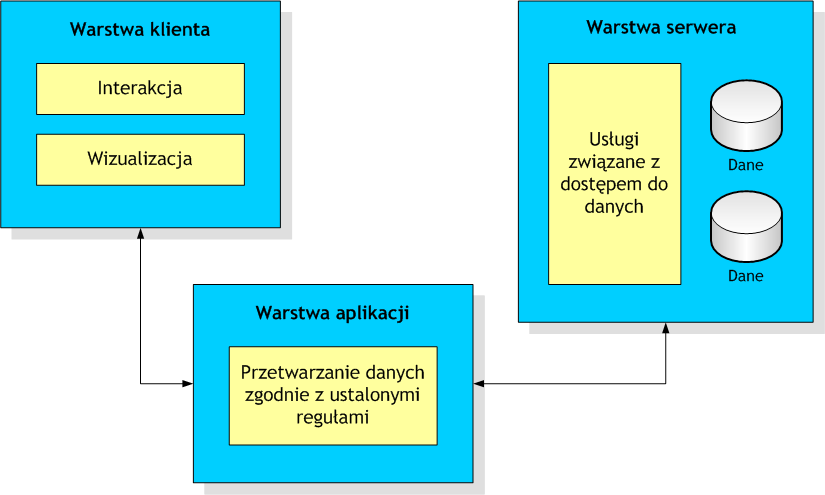
\includegraphics[width=\textwidth]{rys/arch-logiczna.png}
\caption{Architektura logiczna aplikacji}
\label{fig:arch_log}
\end{figure}

Warstwa klienta ma za zadanie wizualizować i prezentować użytkownikowi dane. Poza tym musi pozwalać na interakcję. W takiej postaci klient pełni rolę tzw. forntendu.\newline
Warstwa aplikacji pełni swoisty pomost między bazą danych, a klientem. Ma za zadanie pobierać i przetwarzać dane (np. filtrować, walidować), a także dostarczać nowe porcje danych do bazy danych. Tutaj też powinna znajdować się cała logika biznesowa jak i funkcjonalność odpowiedzialna za liczenie. \newline
Warstwą serwera jest dowolnie wybrana implementacja bazy danych. Ma za zadanie przechowywać dane aplikacji oraz dane kont użytkowników. W tym miejscu można było się pokusić o wybranie nierelacyjnej bazy danych, lecz ostatecznie została wybrana relacyjna.

\section{Architektura fizyczna}
\label{chap:arch_fiz}
Na Rysunku \ref{fig:arch_fiz} został przedstawiony schemat architektury fizycznej aplikacji. Bliźniaczo jak w przypadku architektury logicznej jej struktura narzucona jest wyborami technologii przedstawionych w Rozdziale \ref{chap:technologies}. Składają się one z backendu .NET Core, który używa GraphQL jako standardu API. Zarządza on bazami danych postawionych na PostgreSQL. Rolę klienta pełni środowisko programistyczne Angular posiadające komponenty, które zawierają logikę aplikacji frontendowej i komunikują się z widokami. Poprzez wstrzykiwanie zależności komponenty mają dostęp do wspólnych zasobów i funkcji. Aplikacja klienta posiada również możliwości zapisywania danych w przeglądarce użytkownika w postaci ciasteczek, co może być przydatne przy zapisywaniu aktualnego stanu zalogowanego użytkownika.


\begin{figure}[H]
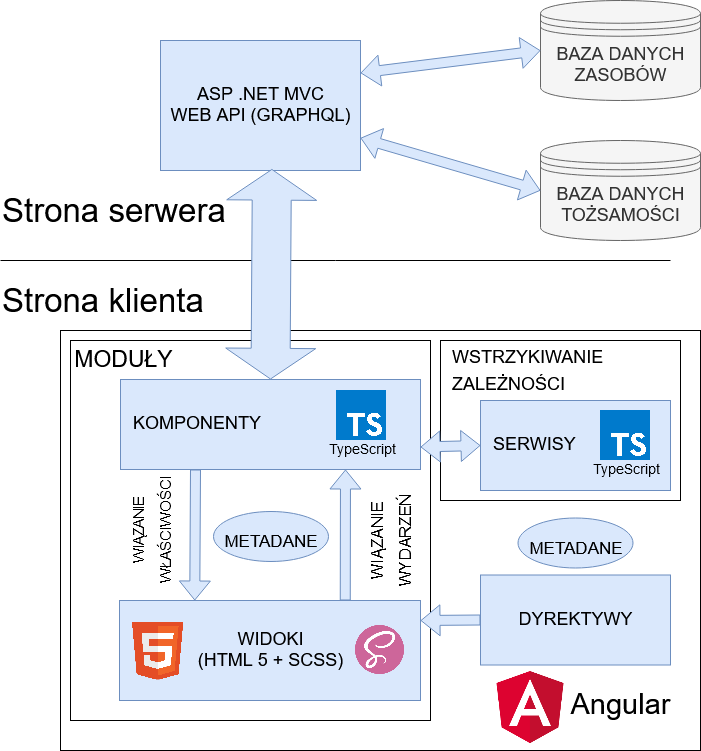
\includegraphics[width=\textwidth]{rys/arch-fiz.png}
\caption{Architektura fizyczna aplikacji}
\label{fig:arch_fiz}
\end{figure}



\chapter{Implementacja}
W tym rozdziale przybliżone zostało działanie aplikacji w odniesieniu do wykorzystywanych technologii.

\section{Stos technologiczny}

Przed przystąpieniem do przeglądu konkretnych rozwiązań i bibliotek, które zostały wykorzystane podczas tworzenia aplikacji. 
\begin{itemize}
    \item Jako platforma programistyczna backendowy został wykorzystany ASP.NET CORE 3.0, w którym można pisać w języku C\#. Nadaje się doskonale do pisania interfejsu programistycznego aplikacji.\cite{asp} Dzięki architekturze MVC można było w sposób zrozumiały i ścisły sposób opisać reguły w jaki programy komunikują się ze sobą.\cite{asp} W skrócie nazywa się to API. Jest ono definiowane już na poziomie kodu źródłowego, a jego zadaniem jest przekazanie wyszczególnionego spisu struktur danych, podprogramów, klas oraz protokołów do komunikacji.\cite{api} Funkcje API są użyczane jako zasób w sieci.
    \item Jako platforma programistyczna frontendowa został wykorzystany Angular w wersji 8.0.0. Został on napisany w języku TypeScript, który jest nadzbiorem języka JavaScript, który został poszerzony o funkcje typowania oraz dopełniające struktury językowe niedostępne w ECMAScript.\cite{ts} ECMAScript jest znormalizowaną specyfikacją skryptowego języka programowania, której implementacją jest między innymi JavaScript. Angular jest otwarty i pozwala na tworzenie SPA, czyli aplikacji jednostronicowej. Jest to aplikacja lub witryna internetowa, która ma możliwość wchodzenia w interakcję z użytkownikiem poprzez dynamiczne przepisywanie bieżącej strony zamiast ładowania całych nowych stron z serwera. Podejście takie pozwala unikać zakłóceń w obsłudze między kolejnymi stronami, dzięki czemu zachowanie programu jest bliższe do okienkowej aplikacji komputerowej. W SPA cały niezbędny kod, czyli HTML, JavaScript i CSS są pobierane przy pojedynczym przeładowaniu strony lub potrzebne zasoby są dynamicznie ładowane, a później dodawane do strony w razie konieczności(zazwyczaj w odpowiedzi na działania użytkownika).\cite{spa}
    \item Jako baza danych wykorzystywany jest PostgreSQL. Jest otwartym systemem zarządzania relacyjnymi bazami danych (DBMS), który został stworzony przez ogólnoświatowy zespół ochotników. Dzięki czemu nie jest kontrolowany przez żadną korporację czy inny podmiot prywatny, a kod źródłowy jest dostępny za darmo dla każdego. PostgreSQL obsługuje między innymi transakcje, podselekcje, wyzwalacze, integralność referencyjną kluczy obcych, widoki.\cite{postgresql}
\end{itemize}
Poniżej opisano wykorzystane narzędzia:
\begin{itemize}
    \item Rider -- zintegrowane środowisko programistyczne, czyli program który udostępnia złożoną funkcjonalność obejmującą tworzenie oprogramowania, przede wszystkim edycję kodu źródłowego oraz jego kompilację. Ponadto umożliwia debugowanie aplikacji oraz integruje się z wykorzystywaną bazą danych. Zostało wydane oraz jest rozwijane przez firmę JetBrains. Środowisko to pozwala na tworzenie różnorakich aplikacji w .NET oraz obsługuję również frameworki frontendowe takie jak Angular oraz React.\cite{rider} Umożliwia również używanie wygodnych skrótów klawiszowych, które w znaczący sposób przyśpieszają pracę nad oprogramowaniem.
    \item TSLint -- jest rozszerzalnym narzędziem do statycznej analizy kodu napisanego w TypeScript pod kątem czytelności, łatwości utrzymania oraz błędów funkcjonalnych. Można go dostosowywać do własnych reguł, konfiguracji i formatów.\cite{tslint}
    \item Git -- jest otwarto-źródłowym rozproszonym systemem kontroli wersji, które służy do monitorowania zmaina w kodzie źródłowym w trakcie tworzenia oprogramowania. Przeznaczony on jest do koordynowania pracy programistów, ale może również służyć do śledzenia dowolnych plików. Git charakteryzuje się szybkością, integralność danych oraz obsługa rozproszonych, nieliniowych przepływów pracy. Został stworzony przez Linusa Torvaldsa w 2005 roku w celu rozwoju jądra Linuksa. Podobnie jak w innych rozproszonych systemach kontroli wersji i w przeciwieństwie do systemów klient-serwer, każdy katalog Git na odrębnych komputerach jest pełnoprawnym repozytorium z zachowaniem pełnej historii i pełnych możliwości śledzenia wersji, niezależnie od dostępu do serwera centralnego.\cite{git}.
\end{itemize}

\section{API}
Zgodnie z architekturą zaprezentowaną w Rozdziale \ref{chap:arch_log} oraz Rozdziale \ref{chap:arch_fiz} API zostało zaimplementowana w następujący sposób.
\subsection{Struktura}
Na Rysunku \ref{fig:struct_api} przedstawiono strukturę backendu, który pełni funkcję interfejsu programistycznego aplikacji.
\begin{figure}[H]
\centering
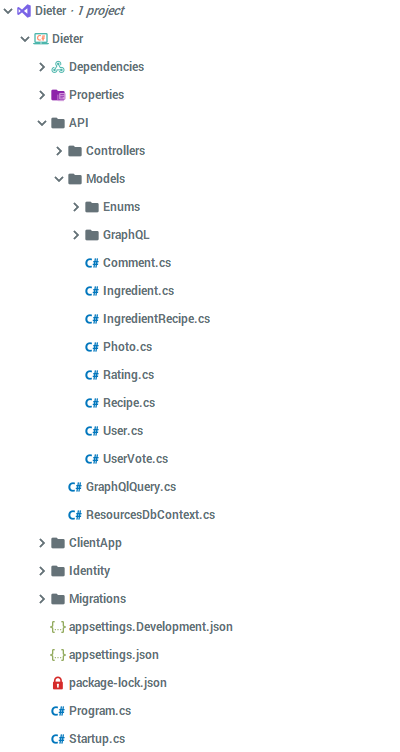
\includegraphics[width=.5\textwidth]{rys/struktura-api.png}
\caption{Struktura API}
\label{fig:struct_api}
\end{figure}

\subsection{Model danych i integracja z bazą danych}
Na początku zostały zdefiniowane modele danych, które później za pomocą biblioteki Entity Framework Core zostały zmapowane do relacyjnej bazy danych. Poniżej przedstawiono przykładowy model.
\begin{lstlisting}[language={[Sharp]C}]
 public class Recipe
    {
        
        public int RecipeId { get; set; }
        public virtual User Author { get; set; }
        public string Name { get; set; }
        public string Description { get; set; }
        public int? Calories { get; set; }
        public int? Weight { get; set; }
        public int? EstTime { get; set; }
        public Difficulty? Difficulty { get; set; }
        public virtual Rating Rating { get; set; }
        
        public virtual ICollection<Comment>
        Comments { get; set; }
        public virtual ICollection<IngredientRecipe>
        IngredientRecipes { get; set; }
    }
\end{lstlisting}
Obiekty domyślnie są mapowane na atrybuty, które mogą zawierać wartość zerową. Typy prymitywne takie jak na przykład \texttt{int} nie posiadają tej właściwości, więc aby w bazie danych mogły być wartością opcjonalną należy dodać znak pytajnika po typie. Modyfikator \texttt{virtual} pozwala na leniwe załadowanie danych, dzięki czemu później wykonując kweredndy GraphQL będzie możliwe swobodne poruszanie się między tabelami. Na podstawie powyższego kodu powstała tabela przedstawiona na Rysunku \ref{fig:recipe_table}. Jak widać oprócz atrybutów zostały utworzone klucze obce do innych tabel.

\begin{figure}[H]
\centering
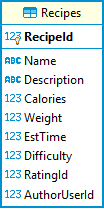
\includegraphics[width=.2\textwidth]{rys/recipe.png}
\caption{Tabela przepisu}
\label{fig:recipe_table}
\end{figure}

Po utworzeniu wszystkich modelów zostały one użyte do zainicjalizowania kontekstu bazy danych, który po połączeniu z bazą danych pozwala na łatwą manipulację danych. Poniżej przedstawiono tworzenie takiego kontekstu.

\begin{lstlisting}[language={[Sharp]C}]
  public ResourcesDbContext(DbContextOptions
  <ResourcesDbContext> options) : base(options)
        {
        }
        protected override void OnModelCreating
        (ModelBuilder modelBuilder)
        {
            modelBuilder.Entity<IngredientRecipe>()
            .HasKey(ir => new {ir.IngredientId, ir.RecipeId});
        }
        
        protected override void OnConfiguring
        (DbContextOptionsBuilder optionsBuilder)
        {
            optionsBuilder.UseLazyLoadingProxies();
        }

        public DbSet<Comment> Comments { get; set; }
        public DbSet<Ingredient> Ingredients { get; set; }
        public DbSet<Rating> Ratings { get; set; }
        public DbSet<Recipe> Recipes { get; set; }
        public DbSet<User> Users { get; set; }
        public DbSet<IngredientRecipe> IngredientRecipes 
        { get; set; }
        public DbSet<UserVote> UserVotes { get; set; }
    }
\end{lstlisting}

Jak widać podano w nim wszystkie utworzone wcześniej modele. Bardzo ciekawym rozwiązaniem jest użycie metody \texttt{r.UseLazyLoadingProxies ( )}, która umożliwia leniwe ładowanie, dzięki czemu można odwoływać się coraz głębiej w obiekty. Znacząco ułatwia to późniejszą pracę. Dodatkowo powiązano ze sobą klucze składniku \texttt{IngredientId} oraz przepisu \texttt{RecipeId} w modelu pośredniczącym \texttt{IngredientRecipe}. Działanie to powoduje stworzenie relacji wiele do wielu, która po wysłaniu struktury do bazy danych będzie w postaci dodatkowej tabeli.\newline

Połączenie z bazą danych było bardzo proste. Wystarczyło wywołać poniższą funkcję oraz zdefiniować w osobnym pliku dane potrzebne do połączenia z bazą danych.
\begin{lstlisting}[language={[Sharp]C}]
 services.AddDbContext<ResourcesDbContext>(opt =>
                opt.UseNpgsql(Configuration
                .GetConnectionString("DefaultConnection")));
\end{lstlisting}
Poniżej znajdują się przykładowe dane potrzebne do połączenia z serwerem PostgreSQL.
\begin{lstlisting}
  "ConnectionStrings": {
    "DefaultConnection": "User ID =postgres;Password=pass;
    Server=localhost;Port=5432;Database=DieterDb;
    Integrated Security=true;Pooling=true;",
  },
\end{lstlisting}

Oprócz modeli danych zostały też stworzone wyliczeniowe typy danych, które są później wykorzystywane w owych modelach. Przykładowy typ wyliczeniowy został przedstawiony poniżej.

\begin{lstlisting}[language={[Sharp]C}]
 public enum Difficulty
    {
        VeryEasy,
        Easy,
        Medium,
        Hard,
        VeryHard,
    }
\end{lstlisting}

\subsection{Kontroler}
Kontroler w API służy do obsługi przychodzących żądań HTTP i odsyła odpowiedź. W aplikacji w sytuacji korzystania ze standardu REST lub SOAP w zdecydowanej większości wypadków będzie występował więcej niż jeden kontroler. Ale ze względu na wykorzystanie w projekcie GraphQL występuje tylko jeden kontroler. Tak wynika ze specyfikacji tego standardu.\cite{gqlcode} Na poniższym listingu znajduje się ten kontroler.
\begin{lstlisting}[language={[Sharp]C}]
[Route("graphql")]
public class GraphQlController : Controller
    {
        private readonly ResourcesDbContext _db;
        private readonly UserManager<AppUser> _userManager;
        private readonly SignInManager<AppUser> _signInManager;

        public GraphQlController(ResourcesDbContext db,
            UserManager<AppUser> userManager,
            SignInManager<AppUser> signInManager)
        {
            _db = db;
            _userManager = userManager;
            _signInManager = signInManager;
        }

        public async Task<IActionResult> 
        Post([FromBody] GraphQlQuery query)
        {
            var inputs = query.Variables.ToInputs();

            var schema = new Schema()
            {
                Query = new DieterQuery(_db),
                Mutation = new DieterMutation
                (_db, _userManager, _signInManager)
            };

            var result = await new DocumentExecuter()
            .ExecuteAsync(_ =>
            {
                _.Schema = schema;
                _.Query = query.Query;
                _.OperationName = query.OperationName;
                _.Inputs = inputs;
            }).ConfigureAwait(false);

            if (result.Errors?.Count > 0)
            {
                return BadRequest();
            }

            return Ok(result);
        }
    }
\end{lstlisting}

Jak widać tworzy schemat na podstawie typów, kwerend oraz mutacji. Następnie zwraca wynik o wcześniej zdefiniowanej strukturze. W razie potrzeby kontroler może zwrócić też błąd. Na samym początku podana jest trasa do połączenia się z danym punktem końcowym, będzie ona potrzebna później w aplikacji klienckiej. 

\subsection{GraphQL}
Na Rysunku \ref{fig:graphql_table} przedstawiono strukturę plików wykorzystaną w projekcie aplikacji.
Dzielą się one na pliki definiujące:
\begin{itemize}
    \item typy, które są tworzone na podstawie modeli oraz typów wyliczeniowych,
    \item typy wejściowe, które są przekazywane jako argumenty do mutacji i kwerend,
    \item kwerendy, które służą do pobierania danych, zawierają w sobie pobieranie danych z serwera, obliczenia i działania na nich oraz mapowanie na odpowiednie typy,
    \item mutacje, które są operacjami modyfikującymi stan danych, czyli edycja, dodawanie oraz usuwanie. Muszą zwrócić jakiś typ tak samo jak kwerenda.
\end{itemize}
Razem tworzą schemat GraphQL, który można traktować jako kontrakt między backendem, a frontendem. Jego wcześniejsze zdefiniowanie pozwala w większych zespołach na bardziej niezależną od siebie pracę. W jednoosobowym projekcie nie ma to aż tak wielkiego znaczenia.

\begin{figure}[H]
\centering
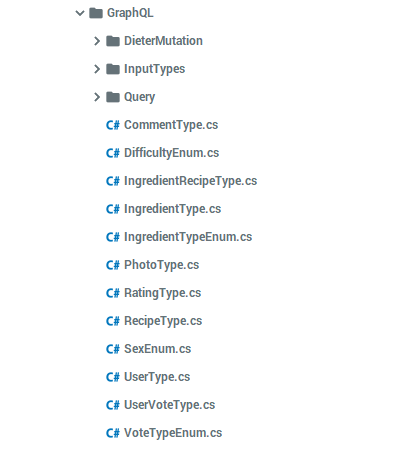
\includegraphics[width=.7\textwidth]{rys/struktura-graphql.png}
\caption{Struktura plików GraphQL}
\label{fig:graphql_table}
\end{figure}

Poniżej znajduje się przykładowa kwerenda GraphQL, która zwraca wszystkie komentarze dla przepisu o podanym jako argument numerze identyfikującym. Dzięki wykorzystaniu Entity Framework Core i języka LINQ, wykonywane jest filtrowanie danych na tabeli \textit{Comments}, szukając rekordów o podanym wcześniej numerze przepisu. Zwrócony typ jest automatycznie mapowany na typ GraohQL.
\begin{lstlisting}[language={[Sharp]C}]
 Field<ListGraphType<CommentType>>(
      "getComments",
       arguments: new QueryArguments(
          new QueryArgument<IdGraphType> {Name = "recipeId"}),
       resolve: context =>
         {
          var recipeId = context.GetArgument<int?>("recipeId");
          return db.Comments
          .Where(x => x.Recipe.RecipeId == recipeId);
      });
\end{lstlisting}

Natomiast na poniższym listingu przedstawiono przykładową mutację. Zostało tu pokazane dodawanie komentarza. Jako argumenty przekazywane są treść komentarza oraz numery identyfikacyjne autora i przepisu, do którego komentarz jest wystawiany. Znowu dzięki użyciu Entity Framework Core w prosty sposób można było wykonać operację na bazie danych. Po edycji obiektu w kodzie, który ma swoje odzwierciedlenie w strukturze bazy danych i wywołaniu metody \texttt{SaveChanges()} na kontekście bazy danych, baza danych zostaje zaktualizowana o przeprowadzone zmiany.

\begin{lstlisting}[language={[Sharp]C}]
Field<CommentType>(
    "addComment",
    arguments: new QueryArguments(
        new QueryArgument<NonNullGraphType
        <AddCommentInputType>> {Name = "comment"},
        new QueryArgument<NonNullGraphType
        <IdGraphType>> {Name = "authorUserId"},
        new QueryArgument<NonNullGraphType
        <IdGraphType>> {Name = "recipeId"}),
    resolve: context =>
    {
        var comment = context.GetArgument<Comment>("comment");
        var authorUserId = context.GetArgument<int>("authorUserId");
        var recipeId = context.GetArgument<int>("recipeId");

        //add rating record
        var rating = new Rating();
        db.Ratings.Add(rating);
        db.SaveChanges();
        comment.Rating = rating;

        //add author
        comment.Author = db.Users
        .FirstOrDefault(x => x.UserId == authorUserId);
        //add recipe
        comment.Recipe = db.Recipes
        .FirstOrDefault(x => x.RecipeId == recipeId);

        //add comment
        comment.PublicationDate = DateTime.Now;
        db.Comments.Add(comment);
        db.SaveChanges();

        return comment;
    });
\end{lstlisting}

\subsection{Identity Core}
Jest to system, który obsługuje funkcje rejestracji oraz logowania użytkownik oraz uwierzytelnianie i autoryzację. Użytkownicy mogą stworzyć konto z danymi, które są zapisywane w odpowiednich tabelach wcześniej wygenerowanej bazy danych lub skorzystać z danych logowania zewnętrznego dostawcy takiego jak na przykład Facebook, Google, Microsoft, Twitter. Jej strukturę przedstawiono na Rysunku \ref{fig:identity_schema}. Przechowywanie tożsamości domyślnie jest skonfigurowane do wykorzystywania SQL Server, ale z powodzeniem można używać innych systemów obsługi baz danych. W aplikacji wykorzystano integrację z PostgreSQL. Implementacja została wykonana dzięki wbudowanej w .NET Core możliwości integracji z aplikacją. Wystarczyło dodanie biblioteki przez menedżer pakietów NuGet oraz krótka konfiguracja.


\begin{figure}[H]
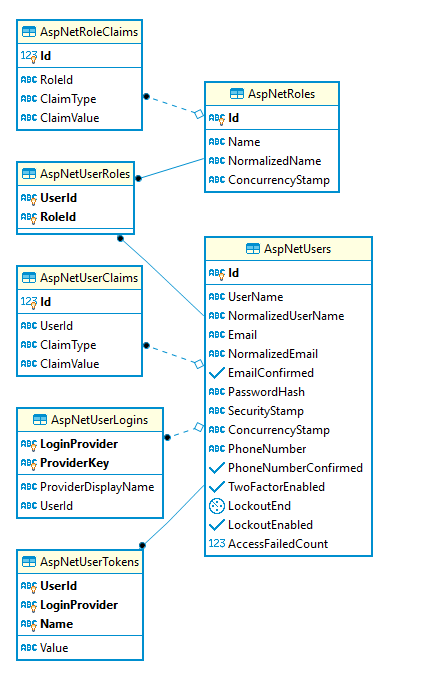
\includegraphics[width=.9\textwidth]{rys/identity-baza.png}
\caption{Schemat bazy danych tożsamości}
\label{fig:identity_schema}
\end{figure}

\section{Aplikacja przeglądarkowa}
Aplikacja przeglądarkowa została napisana z pomocą frameworku Angular i skojarzonych z nim bibliotek. W poniższym rozdziale została opisana jej implementacja. Za Rysunku \ref{fig:front_schem} została przedstawiona struktura projektu.


\begin{figure}[H]
\centering
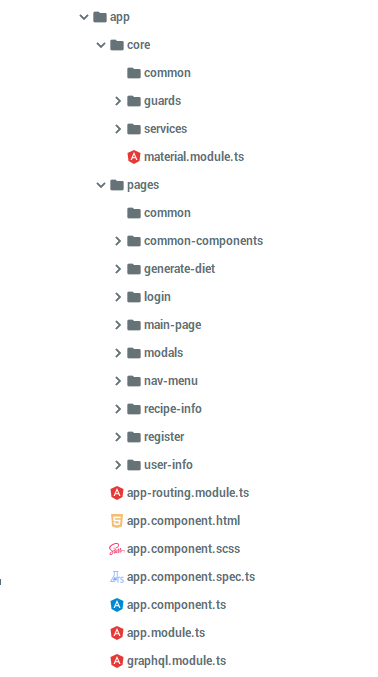
\includegraphics[width=.7\textwidth]{rys/front-schem.png}
\caption{Struktura plików aplikacji przeglądarkowej}
\label{fig:front_schem}
\end{figure}

\subsection{Połączenie z API}
Do połączenia został wykorzystany klient Apollo. Jest to niezwykle elastyczny, oparty na pracy zaangażowanej społeczności klient GraphQL dla platformy Angular.\cite{apollo} Został zaprojektowany, aby ułatwić tworzenie komponentów interfejsu użytkownika, które pobierają dane za pomocą GraphQL. Rozwiązanie to zostało wybrane ponieważ:
\begin{itemize}
    \item przystosowalność -- można wykorzystać go w istniejącej aplikacji,
    \item uniwersalność -- jest kompatybilny z dowolną konfiguracją, dowolnym serwerem lub schematem GraphQL,
    \item nieskomplikowanie -- w łatwy sposób można pobrać dane, a wykorzystaniem dodatkowej, bardziej zaawansowanej funkcjonalności zostawić sobie na później,
    \item zrozumiały i łatwy do sprawdzania,
    \item mały i elastycznym -- nie potrzebuje wielu zasobów do poprawnego działania, a jego rdzeń został skompresowany do rozmiaru poniżej 12 KB,
    \item otwarto-źródłowy -- rozbudowana społeczność trwa o rozwój biblioteki.
\end{itemize}


W poniższym kodzie przedstawiono sposób łączenia się z API. W stałej \texttt{uri} przechowywany jest endpoint backendu. Następnie tworzone jest połączenie poprzez użycie funkcji \texttt{create()} w obiekcie \texttt{httpLink}.
\begin{lstlisting}[language=JavaScript]
const uri = 'https://localhost:5001/graphql';
export function createApollo(httpLink: HttpLink) {
  return {
    link: httpLink.create({uri}),
    cache: new InMemoryCache(),
  };
}

@NgModule({
  exports: [ApolloModule, HttpLinkModule],
  providers: [
    {
      provide: APOLLO_OPTIONS,
      useFactory: createApollo,
      deps: [HttpLink],
    },
  ],
})
export class GraphQLModule {}
\end{lstlisting}

\subsection{Pobieranie danych}
Pobieranie danych w prosty i przewidywalny sposób jest jedną z podstawowych funkcji klienta Apollo.
Na początku należało napisać kwerendę w języku GraphQL. Przykładowa została przedstawiona poniżej. Została tu przedstawiona jedna z ważniejszych zalet GraphQL, a mianowicie możliwość odwoływania się ,,w głąb'' typów danych. Na przykład z poziomu przepisu możemy uzyskać informacje o autorze.
\begin{lstlisting}
query getRecipe($recipeId: ID){
  getRecipe(recipeId: $recipeId){
    recipeId
    description
    calories
    difficulty
    estTime
    weight
    author{
      userName
      userId
    }
    rating{
      downVotes
      upVotes
    }
  }
}
\end{lstlisting}
Następnie na podstawie schematu GraphQL i wcześniej napisanej kwerendy należało wygenerować odpowiednie typy i funkcje zrozumiałe przez język TypeScript. Posłużyło do tego narzędzie graphql-codegen, które na podstawie pliku \texttt{schema.graphql} tworzy wymagane do dalszego działania pliki.\\
Kolejnym krokiem było skorzystanie z mechanizmu wstrzykiwania zależności, czyli dodanie w konstruktorze komponentu obiektu, który z wcześniej wygenerowanych danych jest w stanie komunikować się z API. Przykładowy konstruktor został pokazany poniżej.
\begin{lstlisting}[language=JavaScript]
  constructor(private route: ActivatedRoute,
              private getRecipeGQL: GetRecipeGQL,
              private commonTypes: CommonTypesService,
              private snackBar: MatSnackBar,
              private userService: UserService,
              private voteGQL: VoteGQL,
              private router: Router,
              public dialog: MatDialog) {
  }
\end{lstlisting}
Obiekty z sufiksem \texttt{GQL} odpowiadają za wykonywanie kwerend lub mutacji.\\
Następnym krokiem było pobranie danych, co zostało zobrazowane w poniższej metodzie.
\begin{lstlisting}[language=JavaScript]
  private getRecipe(recipeId: string) {
    this.subscription.add(this.getRecipeGQL
      .fetch({recipeId})
      .subscribe(result => {
        this.loading = result.loading;
        this.recipe = result.data.getRecipe;
      }));
  }
  \end{lstlisting}
  Do zmiennej \texttt{loading} zapisywany jest stan ładowania. Jest on konieczny do wizualizacji procesu pobierania danych. A wszystkie dane dotyczące przepisu przekazywane są do zmiennej \texttt{recipe}, z której później można się bezpośrednio odwoływać w szablonie.
  \subsection{Modyfikacja dancyh}
  Odbywa się w bardzo podobny sposób, co pobieranie danych, schemat praktycznie jest ten sam. Na początku należy napisać mutację, należ
\chapter{Prezentacja aplikacji}
Rozdział  został  poświęcony  prezentacji  zaimplementowanej  aplikacji webowej. Zrzuty ekranu zostały wykonane w przeglądarce Mozilla Firefox 70.0.1.
\section{Logowanie}
Na Rysunku \ref{fig:logowanie} przedstawiono ekran logowania. Jest to pierwsze co zobaczy użytkownik po uruchomieniu aplikacji. Aby przejść dalej należy podać prawidłowe dane logowania lub przejść do formularza rejestracji, aby założyć nowe konto.

\begin{figure}[H]
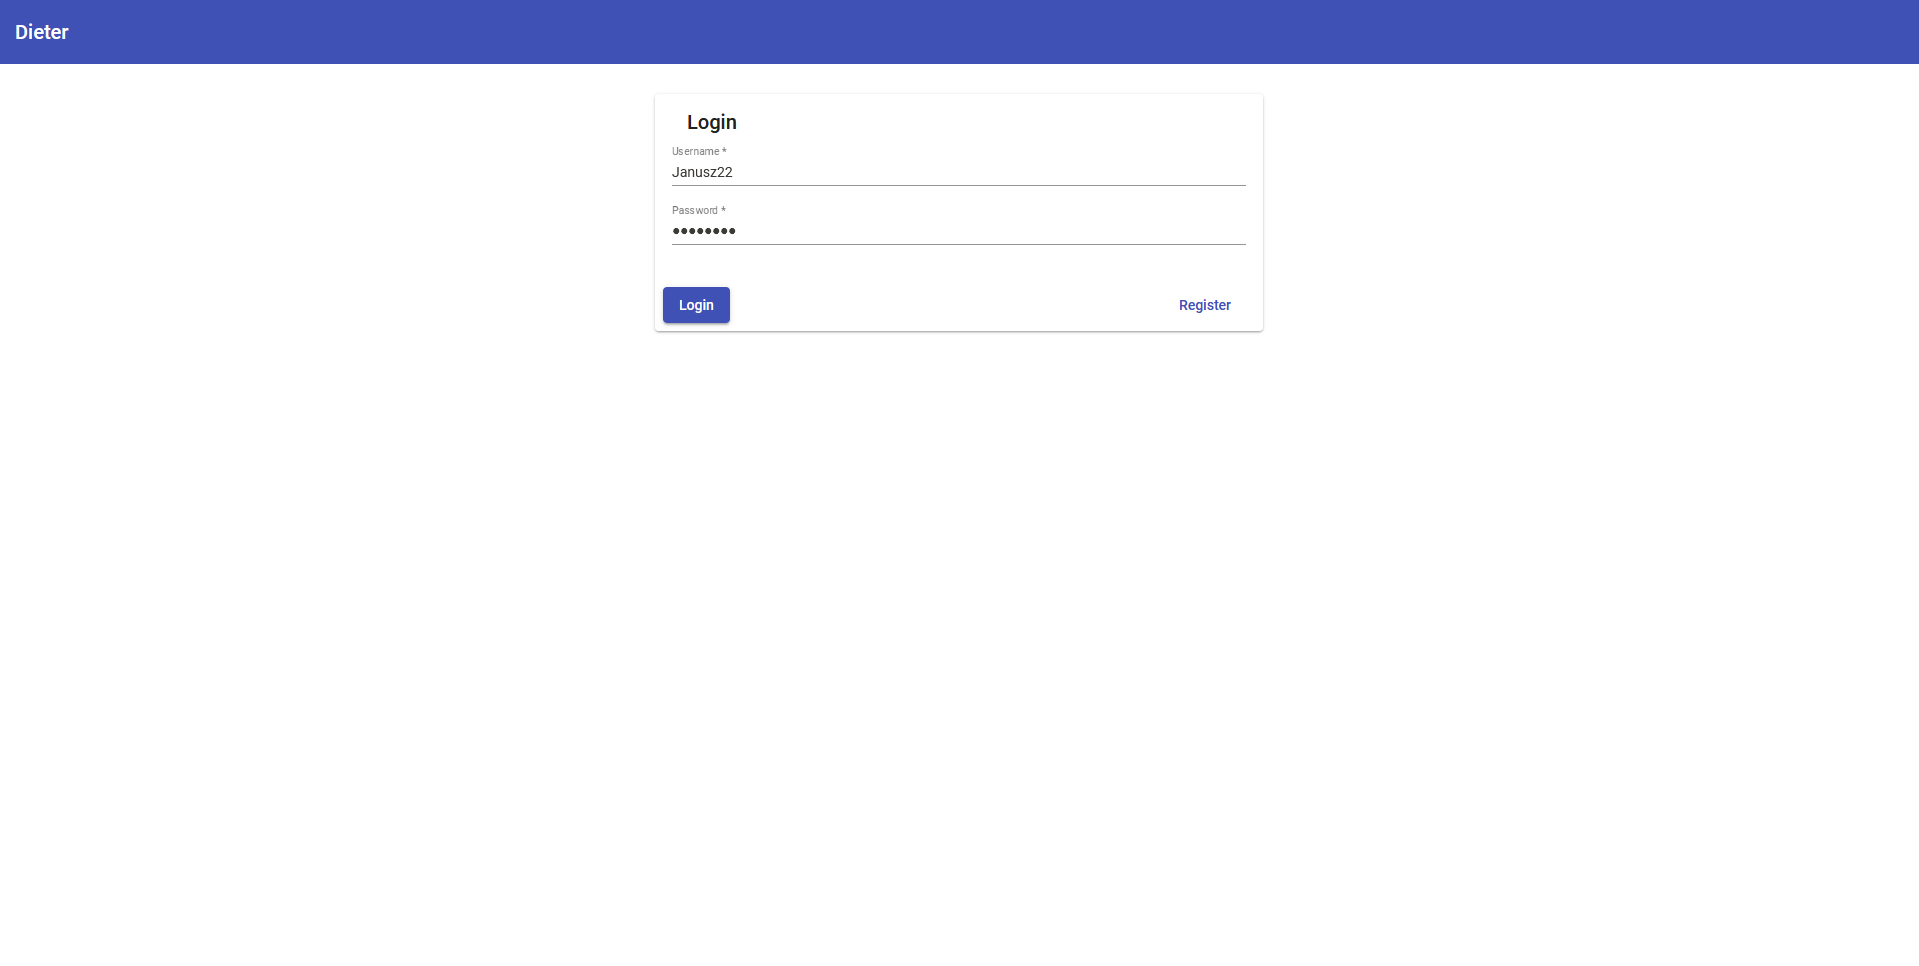
\includegraphics[width=\textwidth]{screeny/logowanie.png}
\caption{Ekran logowania}
\label{fig:logowanie}
\end{figure}

\section{Rejestracja}
Na Rysunku \ref{fig:rejestracja} przedstawiono formularz rejestracji. Aby się zarejestrować należy podać wszystkie wymagane dane w pola. Ich poprawność jest walidowana.

\begin{figure}[H]
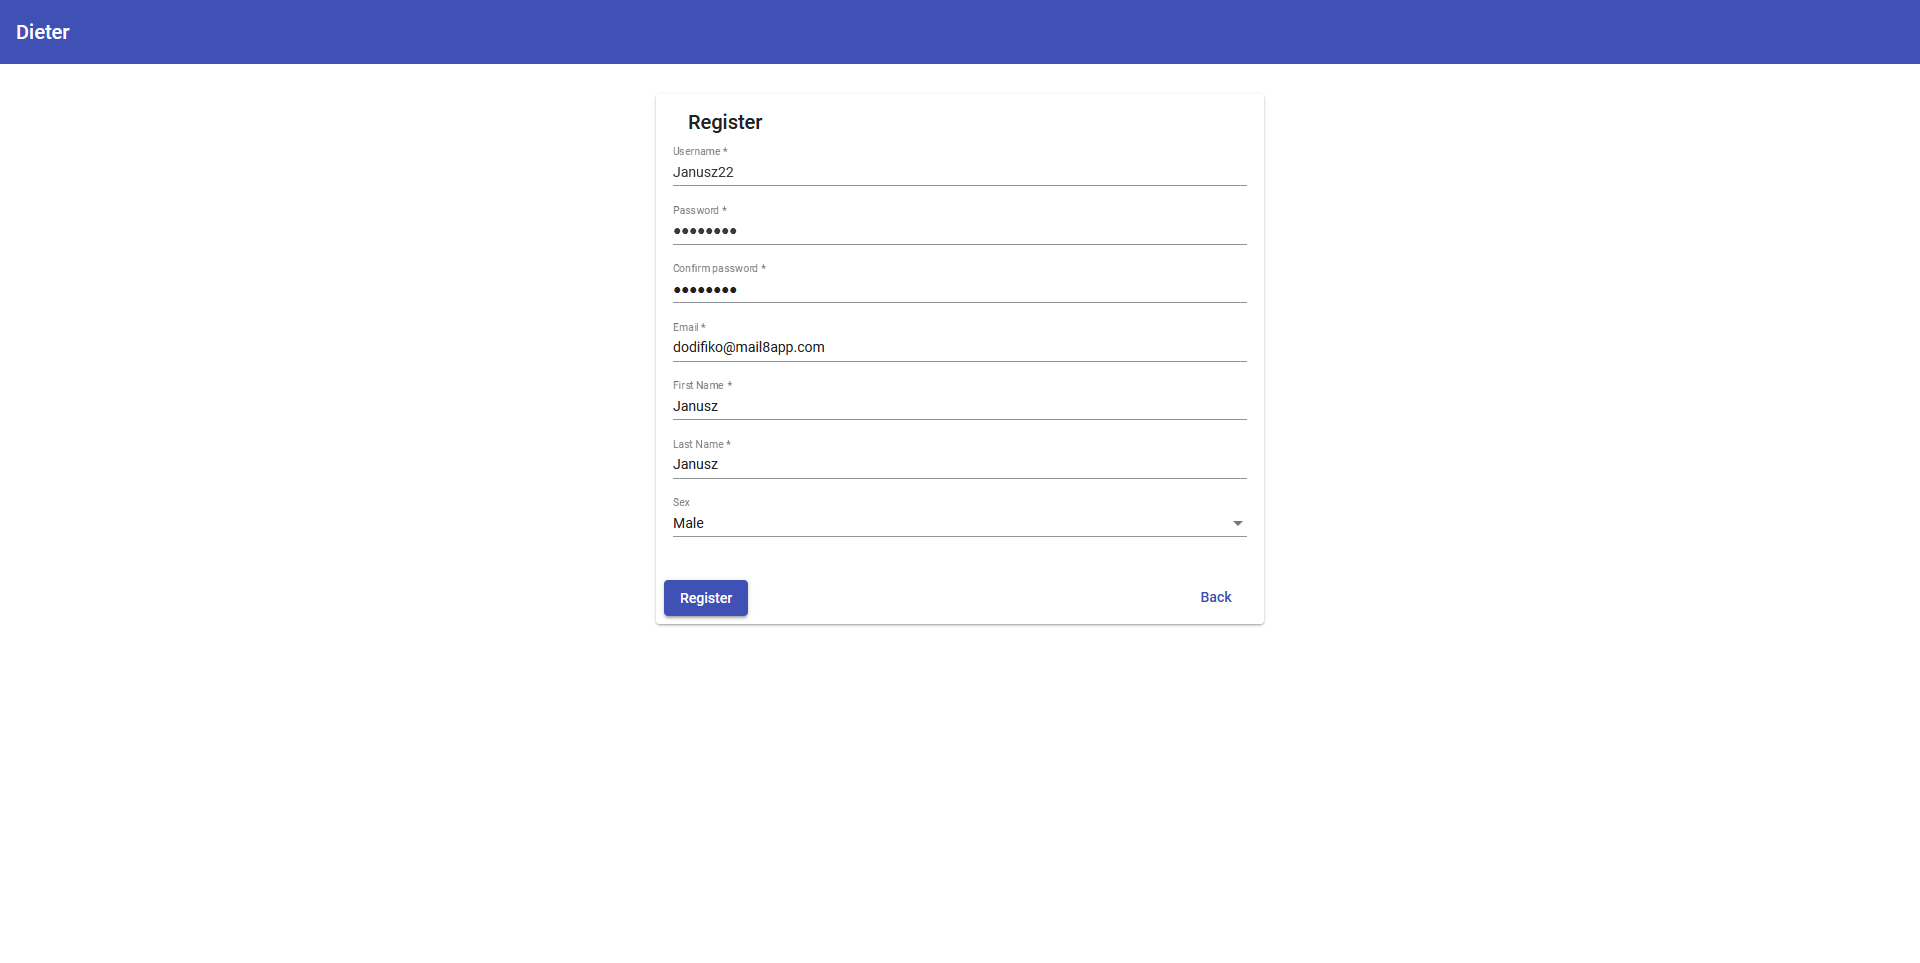
\includegraphics[width=\textwidth]{screeny/rejestracja.png}
\caption{Ekran rejestracji}
\label{fig:rejestracja}
\end{figure}

\section{Generowanie diety}
Na Rysunku \ref{fig:main} przedstawiono ekran generowania diety, a jednocześnie ekran główny aplikacji. Należy podać ilość posiłków, na które ma się składać dieta oraz średnie dzienne zapotrzebowanie kaloryczne. Efekt działania generatora można zobaczyć na Rysunku \ref{fig:use_case}. Po naciśnięciu w przepisu z listy wyświetlą się jego szczegóły. Natomiast po naciśnięciu przycisku \textit{Reset} można wygenerować nową dietę.

\begin{figure}[H]
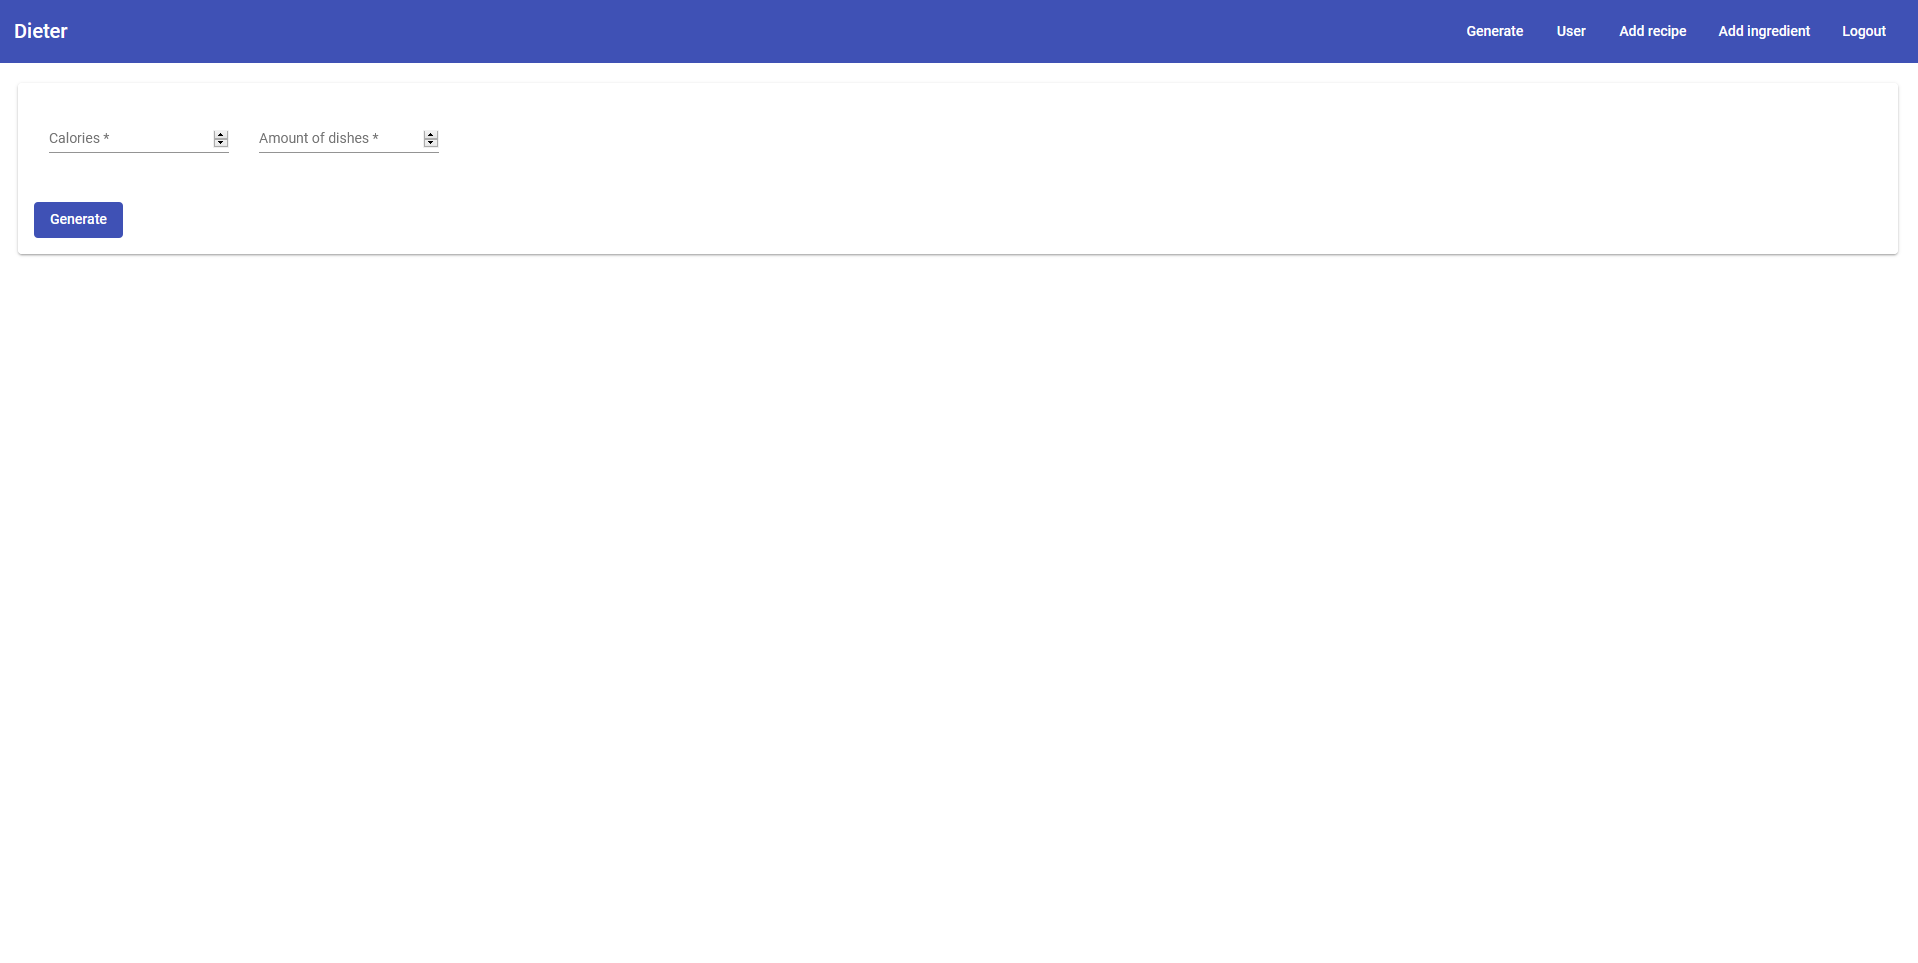
\includegraphics[width=\textwidth]{screeny/main.png}
\caption{Ekran główny}
\label{fig:main}
\end{figure}

\begin{figure}[H]
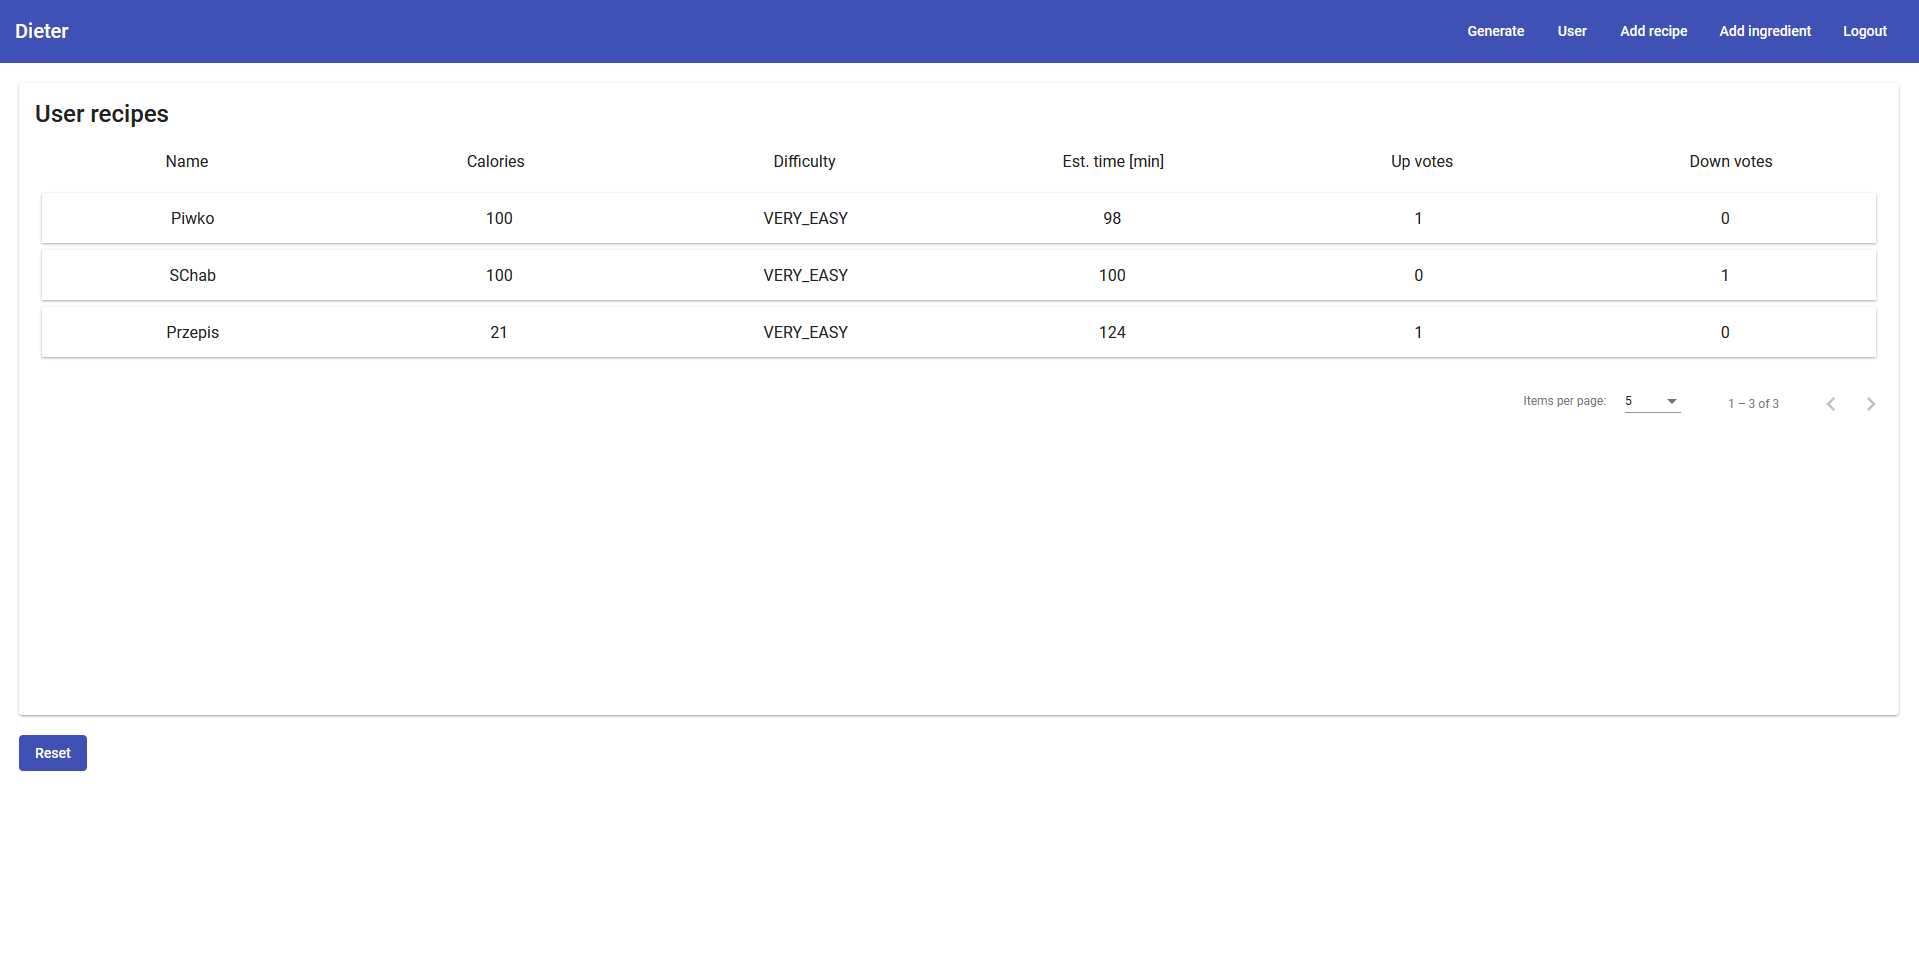
\includegraphics[width=\textwidth]{screeny/generowany.png}
\caption{Wygenerowana dieta}
\label{fig:generowana_dieta}
\end{figure}

\section{Szczegóły użytkownika}
Na Rysunku \ref{fig:user} został pokazany panel szczegółów użytkownika. Widać w nim jego podstawowe informacje oraz listę dodanych przez niego przepisów. Po naciśnięciu w przepisu z listy wyświetlą się jego szczegóły.

\begin{figure}[H]
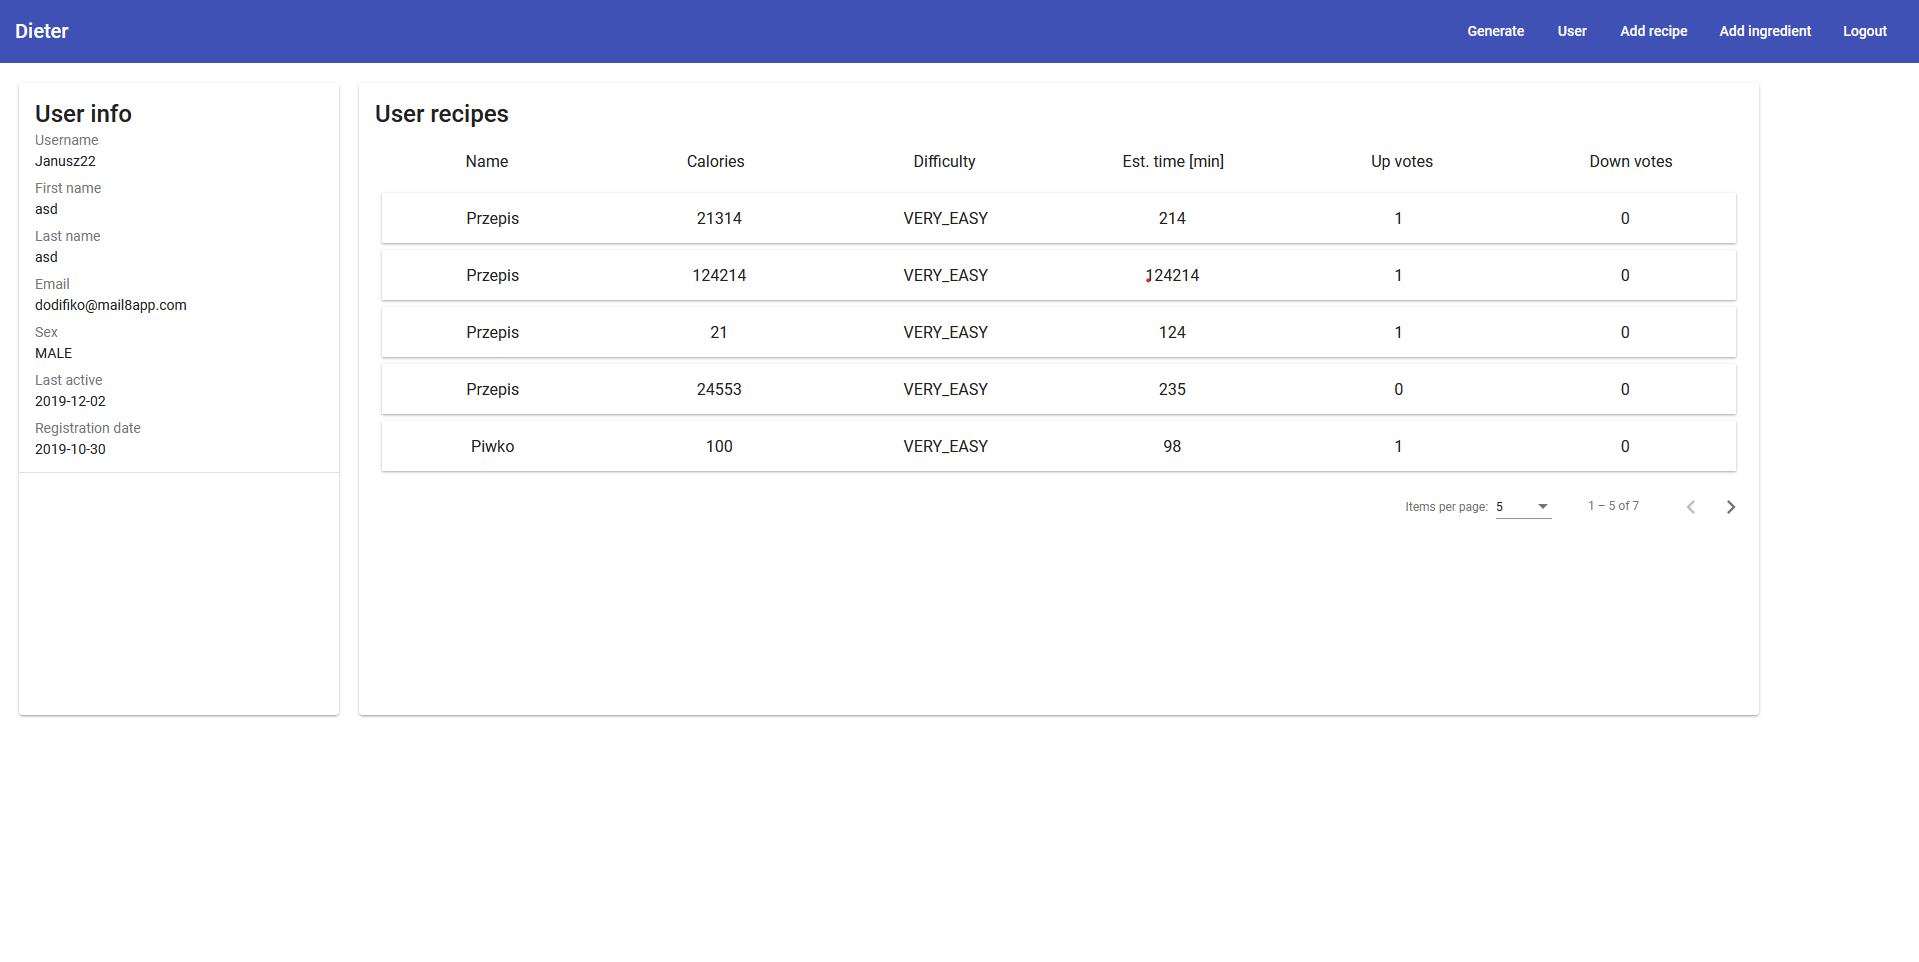
\includegraphics[width=\textwidth]{screeny/user.png}
\caption{Szczegóły użytkownika}
\label{fig:user}
\end{figure}

\section{Dodawanie składnika}
Na Rysunku \ref{fig:ingredient} przedstawiono formularz dodawania składnika. Po wypełnieniu wszystkich wymaganych pól oraz wybraniu kategorii, wystarczy nacisnąć przycisk \textit{Add}.

\begin{figure}[H]
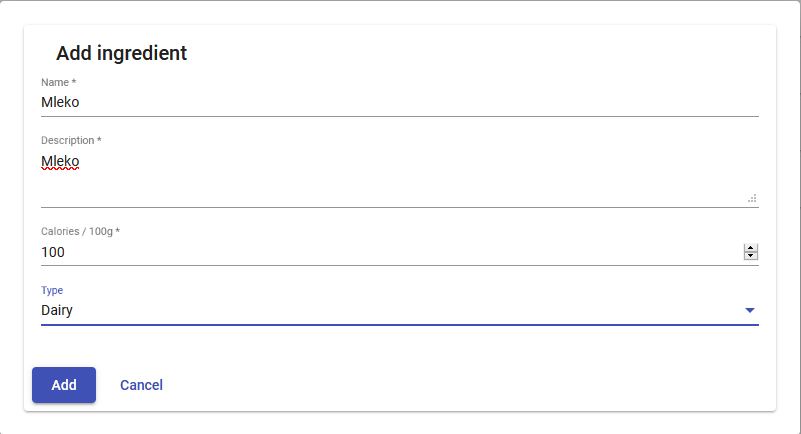
\includegraphics[width=\textwidth]{screeny/dodaj-skladnik.png}
\caption{Dodawanie składnika}
\label{fig:ingredient}
\end{figure}


%\bibliographystyle{plalpha}
\bibliographystyle{plabbrv}

%UWAGA: bibliotekę referencji należy przygotować samemu. Dobrym do tego narzędziem jest JabRef.
%       Nazwę przygotowanej biblioteki wpisuje się poniżej bez rozszerzenia 
%       (w tym przypadku jest to "dokumentacja.bib")
\begin{thebibliography}{9}
    \bibitem{zywienie}
      Agnieszka A. Borowiec, Anita E. Aranowska
      \emph{ Style żywieniowe Polaków i ich społeczno-demograficzne uwarunkowania}.
      Pomeranian J Life Sci, Warszawa
      2018.
    \bibitem{stack}
     \emph{https://insights.stackoverflow.com/survey/2019 }
     Data dostępu: 05.11.2019 09.39
     \bibitem{gqlcode}
     \emph{https://graphql.org/code/}
     Data dostępu: 05.11.2019 15.08
     \bibitem{efcore}
     \emph{https://docs.microsoft.com/pl-pl/ef/core/}
     Data dostępu: 05.11.2019 17:55
     \bibitem{angulararch}
     \emph{https://angular.io/guide/architecture}
     Data dostępu: 05.11.2019 18:37
     \bibitem{analiza}
     Karl E Wiegers, Joy Beatty
     \emph{Specyfikacja oprogramowania. Inżynieria wymagań.}
     Helion,
     2014.
     \bibitem{asp}
     Adam Freeman
     \emph{Pro ASP.NET Core MVC 2}
     APRESS, Londyn
     2019.
     \bibitem{api}
     Glenn Block, Pablo Cibraro, Pedro Felix, Howard Dierking, Darrel Miller
     \emph{Designing Evolvable Web APIs with ASP.NET}
     O'Reilly Media
     2014.
     \bibitem{ts}
     Nathan Rozentals
     \emph{Język TypeScript. Tajniki kodu. Wydanie II}
     Helion,
     2017.
     \bibitem{spa}
     \emph{https://blog.angular-university.io/why-a-single-page-application-what-are-the-benefits-what-is-a-spa/} Data dostępu: 24.11.2019 12:26
     \bibitem{postgresql}
     Joshua D. Drake, John C. Worsley
     \emph{Practical PostgreSQL}
     O'Reilly Media,
     2002.
     \bibitem{rider}
     \emph{https://www.jetbrains.com/rider/}
     Data dostępu: 24.11.2019 12:44
     \bibitem{tslint}
     \emph{https://github.com/palantir/tslint}
     Data dostępu: 24.11.2019 13:00
     \bibitem{git}
     \emph{https://git-scm.com/}
     Data dostępu: 24.11.2019 13:19
     \bibitem{apollo}
     \emph{https://www.apollographql.com/docs/angular/}
     Data dostępu: 01.12.2019 20:50
     \bibitem{scss}
     \emph{https://sass-lang.com/documentation}
     Data dostępu: 02.12.2019 13:46
   
\end{thebibliography}

\newpage
\mbox{}\pdfbookmark[0]{Spis rysunków}{spisRysunkow.1}
%\addcontentsline{toc}{chapter}{Spis rysunków}
\listoffigures*
\begin{flushleft}

\end{flushleft}
%{%
%\let\oldnumberline\numberline%
%\renewcommand{\numberline}{\figurename~\oldnumberline}%
%\listoffigures%
%}


\newpage
\mbox{}\pdfbookmark[0]{Spis tabel}{spisTabel.1}
%\addcontentsline{toc}{chapter}{Spis tabel}
\listoftables*

\appendix
\include{dodatekA}
\include{dodatekB}

\chapterstyle{noNumbered}
\phantomsection % sets an anchor
\addcontentsline{toc}{chapter}{Indeks rzeczowy}
\printindex

\end{document}
